
\documentclass[compress]{beamer}
\mode<presentation>
\usetheme{Warsaw}
\usecolortheme{seagull}
%\useoutertheme[subsection=false]{smoothbars}
\usepackage{fancybox}

\usepackage{stackengine}
%\setbeamertemplate{caption}{\raggedright\insertcaption\par}
\setbeamertemplate{caption}{\insertcaption} 
%\usepackage{caption}



%% ====================================== graphics
\newcommand{\smiley}{\tikz[baseline=-0.75ex,black]{
    \draw circle (2mm);
\node[fill,circle,inner sep=0.5pt] (left eye) at (135:0.8mm) {};
\node[fill,circle,inner sep=0.5pt] (right eye) at (45:0.8mm) {};
\draw (-145:0.9mm) arc (-120:-60:1.5mm);
    }
}

\newcommand{\frownie}{\tikz[baseline=-0.75ex,black]{
    \draw circle (2mm);
\node[fill,circle,inner sep=0.5pt] (left eye) at (135:0.8mm) {};
\node[fill,circle,inner sep=0.5pt] (right eye) at (45:0.8mm) {};
\draw (-145:0.9mm) arc (120:60:1.5mm);
    }
}

\newcommand{\neutralie}{\tikz[baseline=-0.75ex,black]{
    \draw circle (2mm);
\node[fill,circle,inner sep=0.5pt] (left eye) at (135:0.8mm) {};
\node[fill,circle,inner sep=0.5pt] (right eye) at (45:0.8mm) {};
\draw (-135:0.9mm) -- (-45:0.9mm);
    }
}


\usepackage{pgfplots}
\pgfplotsset{width=10cm,compat=1.9}
%\usepgfplotslibrary{external}
%\tikzexternalize
 \usepackage{pgfplotstable}

%\definecolor{markercolor}{RGB}{.49, 1, .63}
\definecolor{markercolor}{RGB}{124.9, 255, 160.65}

\pgfplotsset{
tick label style={font=\scriptsize},
label style={font=\scriptsize},
legend style={font=\scriptsize},
title style={font=\footnotesize}
}

%% ===========================================

\usetikzlibrary{calc}

%%% START MACRO FOR ANNOTATION OF TRIANGLE WITH SLOPE %%%.
\newcommand{\logLogSlopeTriangle}[5]
{
    % #1. Relative offset in x direction.
    % #2. Width in x direction, so xA-xB.
    % #3. Relative offset in y direction.
    % #4. Slope d(y)/d(log10(x)).
    % #5. Plot options.

    \pgfplotsextra
    {
        \pgfkeysgetvalue{/pgfplots/xmin}{\xmin}
        \pgfkeysgetvalue{/pgfplots/xmax}{\xmax}
        \pgfkeysgetvalue{/pgfplots/ymin}{\ymin}
        \pgfkeysgetvalue{/pgfplots/ymax}{\ymax}

        % Calculate auxilliary quantities, in relative sense.
        \pgfmathsetmacro{\xArel}{#1}
        \pgfmathsetmacro{\yArel}{#3}
        \pgfmathsetmacro{\xBrel}{#1-#2}
        \pgfmathsetmacro{\yBrel}{\yArel}
        \pgfmathsetmacro{\xCrel}{\xArel}

        \pgfmathsetmacro{\lnxB}{\xmin*(1-(#1-#2))+\xmax*(#1-#2)} % in [xmin,xmax].
        \pgfmathsetmacro{\lnxA}{\xmin*(1-#1)+\xmax*#1} % in [xmin,xmax].
        \pgfmathsetmacro{\lnyA}{\ymin*(1-#3)+\ymax*#3} % in [ymin,ymax].
        \pgfmathsetmacro{\lnyC}{\lnyA+#4*(\lnxA-\lnxB)}
        \pgfmathsetmacro{\yCrel}{\lnyC-\ymin)/(\ymax-\ymin)} % THE IMPROVED EXPRESSION WITHOUT 'DIMENSION TOO LARGE' ERROR.

        % Define coordinates for \draw. MIND THE 'rel axis cs' as opposed to the 'axis cs'.
        \coordinate (A) at (rel axis cs:\xArel,\yArel);
        \coordinate (B) at (rel axis cs:\xBrel,\yBrel);
        \coordinate (C) at (rel axis cs:\xCrel,\yCrel);

        % Draw slope triangle.
        \draw[#5]   (A)-- %node[pos=0.5,anchor=north] {1}
                    (B)-- 
                    (C)-- node[pos=0.5,anchor=west] {#4}
                    cycle;
    }
}
%%% END MACRO FOR ANNOTATION OF TRIANGLE WITH SLOPE %%%.

%%% START MACRO FOR ANNOTATION OF TRIANGLE WITH SLOPE %%%.
\newcommand{\logLogSlopeTriangleFlip}[5]
{
    % #1. Relative offset in x direction.
    % #2. Width in x direction, so xA-xB.
    % #3. Relative offset in y direction.
    % #4. Slope d(y)/d(log10(x)).
    % #5. Plot options.

    \pgfplotsextra
    {
        \pgfkeysgetvalue{/pgfplots/xmin}{\xmin}
        \pgfkeysgetvalue{/pgfplots/xmax}{\xmax}
        \pgfkeysgetvalue{/pgfplots/ymin}{\ymin}
        \pgfkeysgetvalue{/pgfplots/ymax}{\ymax}

        % Calculate auxilliary quantities, in relative sense.
        %\pgfmathsetmacro{\xArel}{#1}
        %\pgfmathsetmacro{\yArel}{#3}
        \pgfmathsetmacro{\xBrel}{#1-#2}
        \pgfmathsetmacro{\yBrel}{#3}
        \pgfmathsetmacro{\xCrel}{#1}

        \pgfmathsetmacro{\lnxB}{\xmin*(1-(#1-#2))+\xmax*(#1-#2)} % in [xmin,xmax].
        \pgfmathsetmacro{\lnxA}{\xmin*(1-#1)+\xmax*#1} % in [xmin,xmax].
        \pgfmathsetmacro{\lnyA}{\ymin*(1-#3)+\ymax*#3} % in [ymin,ymax].
        \pgfmathsetmacro{\lnyC}{\lnyA+#4*(\lnxA-\lnxB)}
        \pgfmathsetmacro{\yCrel}{\lnyC-\ymin)/(\ymax-\ymin)} % THE IMPROVED EXPRESSION WITHOUT 'DIMENSION TOO LARGE' ERROR.

        \pgfmathsetmacro{\xArel}{\xBrel}
        \pgfmathsetmacro{\yArel}{\yCrel}

        % Define coordinates for \draw. MIND THE 'rel axis cs' as opposed to the 'axis cs'.
        \coordinate (A) at (rel axis cs:\xArel,\yArel);
        \coordinate (B) at (rel axis cs:\xBrel,\yBrel);
        \coordinate (C) at (rel axis cs:\xCrel,\yCrel);

        % Draw slope triangle.
        \draw[#5]   (A)-- node[pos=0.5,anchor=east] {#4}
                    (B)-- 
                    (C)-- %node[pos=0.5,anchor=south] {1}
                    cycle;
    }
}
%%% END MACRO FOR ANNOTATION OF TRIANGLE WITH SLOPE %%%.


\useoutertheme{infolines}
\useinnertheme{rectangles}
\usepackage{hhline}
\setbeamercovered{dynamic}

\usepackage{soul}

\usepackage{array}
\usepackage{amsmath,amssymb,amsfonts,mathrsfs,amsthm}
\usepackage[utf8]{inputenc}
\usepackage{listings}
\usepackage{mathtools}
\usepackage{dsfont}
\usepackage{pdfpages}
%\usepackage[textsize=footnotesize,color=green]{todonotes}
\usepackage{algorithm, algorithmic}
\usepackage{bm}
\usepackage{bbm}

\usepackage{tikz}
\usepackage[normalem]{ulem}

\usepackage{graphicx}
%\usepackage{subfigure}
\usepackage{subfig}
%\usepackage{caption}
%\usepackage{subcaption}

\usepackage{color}
\usepackage{pdflscape}
\usepackage{pifont}

\usepackage{bibentry}
\nobibliography*

%\usepackage[osf]{mathpazo}
%\usepackage{mathpazo}
%\renewcommand\rmdefault{ptm}
\newcommand*\diff[1]{\mathop{}\!{\mathrm{d}#1}}
\renewcommand{\topfraction}{0.85}
\renewcommand{\textfraction}{0.1}
\renewcommand{\floatpagefraction}{0.75}

\newcommand{\vect}[1]{\ensuremath\boldsymbol{#1}}
\newcommand{\tensor}[1]{\underline{\vect{#1}}}
\newcommand{\del}{\triangle}
\newcommand{\grad}{\nabla}
\newcommand{\curl}{\grad \times}
\renewcommand{\div}{\grad \cdot}
\newcommand{\ip}[1]{\left\langle #1 \right\rangle}
\newcommand{\eip}[1]{a\left( #1 \right)}
\newcommand{\td}[2]{\frac{{\rm d}#1}{{\rm d}#2}}
\newcommand{\pd}[3]{\frac{\partial^{#3} #1}{\partial#2^{#3}}}
\newcommand{\pdd}[2]{\frac{\partial^2#1}{\partial#2^2}}

\newcommand{\circone}{\ding{192}}
\newcommand{\circtwo}{\ding{193}}
\newcommand{\circthree}{\ding{194}}
\newcommand{\circfour}{\ding{195}}
\newcommand{\circfive}{\ding{196}}

\newcommand{\Reyn}{\rm Re}

\newcommand{\bs}[1]{\boldsymbol{#1}}
\DeclareMathOperator{\diag}{diag}

\newcommand{\equaldef}{\stackrel{\mathrm{def}}{=}}


\newcommand{\mb}[1]{\mathbf{#1}}
\newcommand{\mbb}[1]{\mathbb{#1}}
\newcommand{\mc}[1]{\mathcal{#1}}
\newcommand{\nor}[1]{\left\| #1 \right\|}
\newcommand{\snor}[1]{\left| #1 \right|}
\newcommand{\Grad} {\ensuremath{\nabla}}
\newcommand{\Div} {\ensuremath{\nabla\cdot}}
\newcommand{\Nel} {\ensuremath{{N^\text{el}}}}
\newcommand{\jump}[1] {\ensuremath{\LRs{\![#1]\!}}}
\newcommand{\avg}[1] {\ensuremath{\LRc{\!\{#1\}\!}}}

\newcommand{\uh}{\widehat{u}}
\newcommand{\fnh}{\widehat{f}_n}
\renewcommand{\hat}{\widehat}
\renewcommand{\L}{L^2\LRp{\Omega}}
\newcommand{\pO}{\partial\Omega}
\newcommand{\Gh}{\Gamma_h}
\newcommand{\Gm}{\Gamma_{-}}
\newcommand{\Gp}{\Gamma_{+}}
\newcommand{\Go}{\Gamma_0}
\newcommand{\Oh}{\Omega_h}

%\newcommand{\nor}[1]{\left\| #1 \right\|}
%\newcommand{\snor}[1]{\left| #1 \right|}
\newcommand{\LRp}[1]{\left( #1 \right)}
\newcommand{\LRs}[1]{\left[ #1 \right]}
\newcommand{\LRa}[1]{\left\langle #1 \right\rangle}
\newcommand{\LRb}[1]{\left| #1 \right|}
\newcommand{\LRc}[1]{\left\{ #1 \right\}}



\newcommand{\bibfoot}[1]{\footnote{\tiny\bibentry{#1}}}
\renewcommand{\note}[1]{\textcolor{red}{{#1}}}

\newcommand{\eval}[2][\right]{\relax
  \ifx#1\right\relax \left.\fi#2#1\rvert}

\def\etal{{\it et al.~}}


\def\arr#1#2#3#4{\left[
\begin{array}{cc}
#1 & #2\\
#3 & #4\\
\end{array}
\right]}
\def\vecttwo#1#2{\left[
\begin{array}{c}
#1\\
#2\\
\end{array}
\right]}
\def\vectthree#1#2#3{\left[
\begin{array}{c}
#1\\
#2\\
#3\\
\end{array}
\right]}
\def\vectfour#1#2#3#4{\left[
\begin{array}{c}
#1\\
#2\\
#3\\
#4\\
\end{array}
\right]}

\newcommand{\G} {\Gamma}
\newcommand{\Gin} {\Gamma_{in}}
\newcommand{\Gout} {\Gamma_{out}}

%\newcommand\blfootnote[1]{%
%  \begingroup
%  \renewcommand\thefootnote{}\footnote{#1}%
%  \addtocounter{footnote}{-1}%
%  \endgroup
%}

% removes nav symbols
\beamertemplatenavigationsymbolsempty
%\setbeamertemplate{caption}{\raggedright\insertcaption\par}

% defines newblock as null, giving compile issues otherwise
\let\newblock\relax 


\title[Multi-patch IGA]{Efficient explicit solvers for multipatch discontinuous Galerkin isogeometric analysis}
\date[June 9-15, 2018]{ECCM-ECFD 2018\\June 9-15, 2018}
\author[Chan, Evans]{Jesse Chan\inst{1}, J. A. Evans\inst{2}}
\institute[Rice CAAM]{\inst{1}Department of Computational and Applied Math, Rice University\\ \inst{2} Ann and H.J. Smead Aerospace Engineering Sciences, UC Boulder}

\begin{document}

\begin{frame}
\maketitle
\end{frame}


\frame{
\frametitle{High order methods for hyperbolic PDEs}
\setcounter{subfigure}{0}
\vspace{-1em}
\begin{columns}
\begin{column}{.5\textwidth}
\begin{itemize}
\item<1-> Time-dependent solutions of hyperbolic equations. 
\vspace{.5em}
\item<2-> Low numerical dissipation and dispersion.
\vspace{.5em}
\item<4-> High order approximations: more accurate per unknown.
\vspace{.5em}
\item<5-> High performance on many-core (explicit time-stepping).
\end{itemize}
\end{column}
\begin{column}{.475\textwidth}
\begin{figure}
\centering
\begin{overlayarea}{\textwidth}{.5\textheight}
\only<1>{
\vspace{-2em}\includegraphics[width=.95\textwidth]{figs/wave.png}
\caption*{Figure courtesy of Axel Modave.}
}
%\only<2>{
%\vspace{1em}
%\includegraphics[width=.95\textwidth]{figs/turbulent1.png}\\
%\vspace{1em}
%\includegraphics[width=.95\textwidth]{figs/turbulent2.png}
%\caption*{Figure courtesy of Per-Olof Persson.}
%}
\only<2>{
\includegraphics[width=.95\textwidth]{figs/wave_N1.eps}
\caption*{\textbf{Fine} linear approximation.}
}
\only<3-4>{
\includegraphics[width=.95\textwidth]{figs/wave_N2.eps}
\caption*{\textbf{Coarse} quadratic approximation.}
}
\only<5>{
\includegraphics[width=.975\textwidth]{figs/gpu.pdf}
\caption*{A graphics processing unit (GPU).}
}
%\caption*{Image courtesy of Axel Modave.}
\end{overlayarea}
\end{figure}
\end{column}
\end{columns}
}

\frame{
\frametitle{Multi-patch discontinuous Galerkin formulations}
\begin{columns}
\begin{column}{.5\textwidth}
\begin{itemize}
\item Wave propagation problems (acoustics, Maxwells, elasticity).
\vspace{.1em}
%\begin{align*}
%%\only<1>{
%\frac{1}{c^2}\pdd{p}{t}{} - \Delta p &= f.
%%}
%%\only<2>{
%%\pd{v}{t}{} &= \sum_{D^k}\LRp{\Grad p,\grad w}_{D^k} + \LRa{\jump{p},w}\\
%%\pd{p}{t}{} &= v.
%%}
%\end{align*}
\item Model problem: acoustic wave equation (both first and second order formulations)
\begin{align*}
\frac{1}{c^2}\pd{p}{t}{} + \Div \bm{u} &= f\\
\pd{\bm{u}}{t}{} + \Grad p &= 0.
\end{align*}
%\item Results extend to second order formulation. 
%\item Multiple geometric patches,\\IGA on each patch.  
\end{itemize}
\end{column}

\begin{column}{.5\textwidth}
\begin{figure}
\centering
\includegraphics[width=\textwidth]{figs/multipatch_diagram.pdf}
\end{figure}
\end{column}

\end{columns}

\vspace{1em}
\begin{itemize}
\item Multiple geometric patches, weak patch coupling through DG-like numerical interface flux (SIPG, upwind).  
\end{itemize}

\let\thefootnote\relax\footnotetext{\tiny Langer et al (2014). \textit{Multipatch discontinuous Galerkin isogeometric analysis}.}
\let\thefootnote\relax\footnotetext{\tiny Wilcox et al (2010). \textit{A high-order DG method for wave propagation through coupled elastic-acoustic media}.}
}

\frame{
\frametitle{Explicit solvers for multi-patch DG-IGA}
%\vspace{-1em}
\begin{itemize}
\item Semi-discrete system:
\[
\bm{M}_h\td{\bm{u}}{t} = \bm{A}_h\bm{u} \quad \Rightarrow \quad \td{\bm{u}}{t} = \bm{M}_h^{-1}\bm{A}_h\bm{u}.
\]
\vspace{.125em}
\item Global mass matrix $\bm{M}_h$ is (patch) block diagonal.  
\vspace{1.5em}
\item Challenges and questions: 
\vspace{.5em}
\begin{itemize}
\item<2-> How to efficiently invert 3D patch mass matrices while guaranteeing accuracy and \textcolor{red}{stability} (especially for explicit methods)?  
\vspace{.5em}
\item<3-> Do splines/IGA offer advantages over $C^0$-FEM/DG for explicit solvers?  
\vspace{.5em}
\item<4-> Can we tailor IGA discretizations towards explicit time-stepping?
\end{itemize}

%\vspace{1em}
%\item Explicit time-stepping, curved domains. 
%%\vspace{.25em}
%\begin{itemize}
%\item Efficient mass matrix inversion over each patch.
%\vspace{.5em}
%\item High order accuracy, energy stability on curved geometries.
%\vspace{.5em}
%\item Improved stable timestep restriction (CFL).
%\end{itemize}
\end{itemize}
}

\section{Inverting IGA mass matrices }
\frame[noframenumbering]{
\frametitle{Outline}
\only<1>{
\tableofcontents
}
\only<2>{
\tableofcontents[currentsection]
}
}

\frame{
\frametitle{B-splines: assumptions for this talk}

\begin{itemize}
\item Reference coordinates $\hat{\bm{x}} \in \hat{D}$, physical coordinates $\bm{x} \in D^k$.  
\vspace{.5em}
\item Standard 1D B-splines: $B^0_i(\hat{x}) = \mathbbm{1}_{\xi_i \leq \hat{x} \leq \xi_{i+1}}$, 
\[
B^k_i(\hat{x}) = \frac{\hat{x} - \xi_i}{\xi_{i+p}-\xi_i}B^{k-1}_i(\hat{x}) + \frac{\xi_{i+p+1}-\hat{x}}{\xi_{i+p+1}-\xi_{i+1}}B^{k-1}_{i+1}(\hat{x}).
\]
\item Physical basis: mapping of tensor product basis on reference domain
%\begin{overlayarea}{\textwidth}{.17\textheight}
\[
%\only<1>{
B^p_{ijk}(\hat{\bm{x}}) = B^p_{i}(\hat{x})B^p_{j}(\hat{y})B^p_{k}(\hat{z}).%, \qquad \text{(mapped B-splines)}}
%\only<2>{B^p_{ijk}({\bm{x}}) = \frac{B^p_{i}(\hat{x})B^p_{j}(\hat{y})B^p_{k}(\hat{z})}{w_R(\hat{\bm{x}})}, \qquad \text{(NURBS)}}
\]
%\end{overlayarea}
\item Assume maximally continuous, open knot vectors
\begin{align*}
%\bm{\Xi} &= \LRc{-1 = \xi_1,\ldots,\xi_{{2p}+K+1} = 1}, \qquad \xi_i \leq \xi_{i+1},\\
\xi_{p+1} &< \ldots < \xi_{p+1+K},\\
\xi_1 &= \ldots = \xi_{p+1},\\
\xi_{p+1 + K} &= \ldots = \xi_{2p+1+K}.\\
\end{align*}
\end{itemize}
}


\frame{
\frametitle{IGA mass matrices: stability/accuracy vs efficiency}

\begin{itemize}
\item Energy stability: if \note{$\bm{u}^T\bm{A}_h\bm{u} \leq 0$}, semi-discrete solution won't blow up
\[
\bm{M}_h\td{\bm{u}}{t} = \bm{A}_h\bm{u} \quad \Longrightarrow \quad \td{}{t}\LRp{\bm{u}^T\bm{M}_h \bm{u}} =  \frac{1}{2}\pd{}{t}{}\nor{u}_{L^2}^2 \leq 0.
\]
\item Approximating $\bm{M}_h^{-1}$ impacts semi-discrete \textcolor{red}{stability} and \textcolor{red}{accuracy}.  
\vspace{2em}
\item<2-> Curved patch mass matrices $\bm{M}_J$: tensor product basis $B^p_{ijk}(\hat{\bm{x}})$
\begin{overlayarea}{\textwidth}{.185\textheight}
\[
\only<1-2>{\LRp{\bm{M}_J}_{ijk,lmn} = \int_{\widehat{D}} B^p_{ijk}(\widehat{\bm{x}})B^p_{lmn}(\widehat{\bm{x}}) \textcolor{red}{J(\widehat{\bm{x}})}\diff{\widehat{\bm{x}}}, \qquad \text{(B-splines)}}
\only<3>{\LRp{\bm{M}_J}_{ijk,lmn} = \int_{\widehat{D}} \frac{B^p_{ijk}(\widehat{\bm{x}})}{\textcolor{red}{w_R\LRp{\hat{\bm{x}}}}}\frac{B^p_{lmn}(\widehat{\bm{x}})}{\textcolor{red}{w_R\LRp{\hat{\bm{x}}}}} \textcolor{red}{{J(\widehat{\bm{x}})}}\diff{\widehat{\bm{x}}} \qquad \text{(NURBS)}}
\only<4>{\LRp{\bm{M}_J}_{ijk,lmn} = \int_{\widehat{D}} B^p_{ijk}(\widehat{\bm{x}})B^p_{lmn}(\widehat{\bm{x}}) \textcolor{red}{\frac{J(\widehat{\bm{x}})}{w^2_R\LRp{\hat{\bm{x}}}}}\diff{\widehat{\bm{x}}} \qquad \text{(NURBS)}}
\]
\end{overlayarea}
\item<2-> No Kronecker structure due to $J(\widehat{\bm{x}})$: $\bm{M}_h$ \textcolor{red}{expensive} to invert in 3D!

\end{itemize}
}

\frame{
\frametitle{Approximate mass matrix inversion}

\begin{itemize}
\item Mass lumping: loss of high order accuracy for IGA.
\vspace{.75em}
\item Preconditioning: 
\vspace{.35em}
\begin{itemize}
\item Additional cost and complexity for a time-domain code.
\vspace{.35em}
\item Semi-discrete stability requires approximation of $\bm{M}_J^{-1}$ to induce a norm on $\bm{u}$ (e.g.\ a fixed symmetric positive-definite linear operator).
\vspace{.35em}
\item Example: Krylov methods approximate $\bm{M}_J^{-1}$ as a non-linear operator!
\end{itemize}
\vspace{.75em}
\item Isogeometric collocation: restores tensor product structure, but semi-discrete stability is more difficult to prove.  
\end{itemize}

\let\thefootnote\relax\footnotetext{\tiny Gao and Calo (2014). \textit{Fast isogeometric solvers for explicit dynamics}.}
\let\thefootnote\relax\footnotetext{\tiny Evans, Hiemstra, Hughes, Reali (2017).  \textit{Explicit higher-order accurate IG collocation methods for structural dynamics}.}
\let\thefootnote\relax\footnotetext{\tiny Wathen and Rees (2009). \textit{Chebyshev semi-iteration in preconditioning for problems including the mass matrix}.}
\let\thefootnote\relax\footnotetext{\tiny Auricchio et al (2012). \textit{Isogeometric collocation for elastostatics and explicit dynamics}.}
}


\frame{
\frametitle{An energy stable and efficient approximation to $\bm{M}^{-1}$}

\begin{itemize}
\item Replace $\bm{M}_J$ with symmetric pos-def ``weight-adjusted'' approximation:
\[
%\td{}{t}
 \bm{M}_J\bm{u} \Rightarrow %\td{}{t}
 \textcolor{red}{\widehat{\bm{M}}\bm{M}_{1/J}^{-1}\widehat{\bm{M}}} \bm{u}, \qquad \LRp{\widehat{\bm{M}}}_{ijk,lmn} = \int_{\widehat{D}} B^p_{ijk}(\widehat{\bm{x}})B^p_{lmn}(\widehat{\bm{x}})\diff{\widehat{\bm{x}}}.
\]
%\vspace{.5em}
\item Weight-adjusted inverse: Kronecker product, matrix-free eval.\ of $\bm{M}_{1/J}$
\begin{align*}
\bm{M}^{-1}_J &\approx \LRp{\widehat{\bm{M}}\bm{M}_{1/J}^{-1}\widehat{\bm{M}}}^{-1}  = \widehat{\bm{M}}^{-1} \bm{M}_{1/J} \widehat{\bm{M}}^{-1}\\
\widehat{\bm{M}}^{-1} &= \widehat{\bm{M}}^{-1}_{\rm 1D} \otimes \widehat{\bm{M}}^{-1}_{\rm 1D} \otimes \widehat{\bm{M}}^{-1}_{\rm 1D}.
\end{align*}
\item Energy stability with respect to an \note{equivalent} norm 
\[
C_1(J) \nor{\bm{u}}_{\widehat{\bm{M}}\bm{M}_{1/J}^{-1}\widehat{\bm{M}}} \leq \nor{\bm{u}}_{\bm{M}_J} \leq C_2 \nor{\bm{u}}_{\widehat{\bm{M}}\bm{M}_{1/J}^{-1}\widehat{\bm{M}}}.
\]
\end{itemize}

\let\thefootnote\relax\footnotetext{\tiny Chan, Hewett, Warburton (2016).  \textit{Weight-adjusted DG methods: wave prop.\ in heterogeneous media}. }
\let\thefootnote\relax\footnotetext{\tiny Chan, Hewett, Warburton (2016).  \textit{Weight-adjusted DG methods: curvilinear meshes}. }
}

\frame{
\frametitle{Accuracy: weighted vs weight-adjusted mass matrix}

\begin{figure}
\centering
\only<1>{
\subfloat[Warped mesh]{\includegraphics[width=.425\textwidth]{figs/mapped.png}}
\subfloat[Error for acoustics (first order form)]{
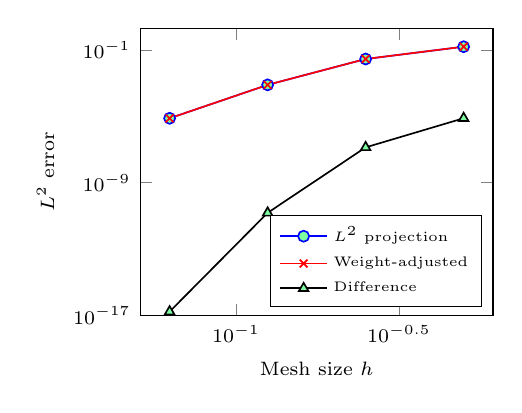
\begin{tikzpicture}
\begin{loglogaxis}[
    legend cell align=left,
    legend style={legend pos=south east, font=\tiny},
    width=.5\textwidth,
     ymin=1e-17, ymax=2,    
    xlabel={Mesh size $h$},
    ylabel={$L^2$ error}, 
    grid style=dashed,
] 
\addplot[color=blue,mark=*,semithick, mark options={solid,fill=markercolor}]
coordinates{(0.5,0.154255)(0.25,0.0280139)(0.125,0.000775805)(0.0625,7.51259e-06)};
\addplot[color=red,mark=x,semithick, mark options={solid,fill=markercolor}]
coordinates{(0.5,0.154523)(0.25,0.0280342)(0.125,0.000775107)(0.0625,7.51217e-06)};
\addplot[color=black,mark=triangle*,semithick, mark options={solid,fill=markercolor}]
coordinates{(0.5,7.56052e-06)(0.25,1.32834e-07)(0.125,1.51285e-11)(0.0625,1.69165e-17)};

\legend{$L^2$ projection,Weight-adjusted,Difference}
%\legend{Uniform, Optimal, Smoothed}
\end{loglogaxis}
\end{tikzpicture}
}
%\subfloat[$L^2$ errors ]{
%\begin{tikzpicture}
%\begin{loglogaxis}[
%    legend cell align=left,
%    legend style={legend pos=south east, font=\tiny},
%    width=.5\textwidth,
%    xlabel={Mesh size $h$},
%    ylabel={$L^2$ error}, 
%             ymin=1e-10, ymax=2,    
%    grid style=dashed,
%] 
%\addplot[color=blue,mark=*,semithick, mark options={solid,fill=markercolor}]
%coordinates{(0.5,0.0110908)(0.25,0.00138298)(0.125,2.29018e-05)(0.0625,3.18561e-07)};
%\addplot[color=red,mark=x,semithick, mark options={solid,fill=markercolor}]
%coordinates{(0.5,0.0111346)(0.25,0.00138582)(0.125,2.30061e-05)(0.0625,3.18565e-07)};
%\addplot[color=black,mark=triangle*,semithick, mark options={solid,fill=markercolor}]
%coordinates{(0.5,0.000986363)(0.25,8.87776e-05)(0.125,2.18816e-06)(0.0625,1.65013e-09)};
%\legend{$L^2$ projection,Weight-adjusted,Difference}
%%\legend{Uniform, Optimal, Smoothed}
%\end{loglogaxis}
%\end{tikzpicture}}
}
\only<2>{
\subfloat[Warped mesh]{\includegraphics[width=.425\textwidth]{figs/mapped2.png}}
\subfloat[Error for acoustics (first order form)]{
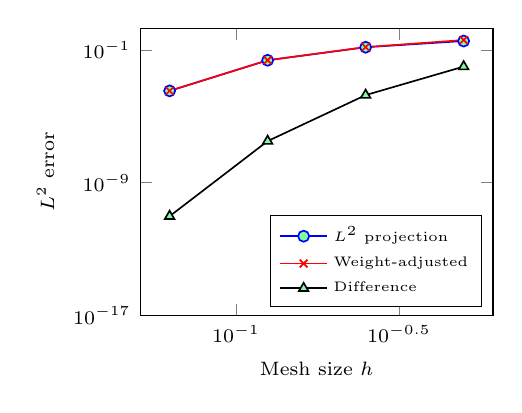
\begin{tikzpicture}
\begin{loglogaxis}[
    legend cell align=left,
    legend style={legend pos=south east, font=\tiny},
    width=.5\textwidth,
     ymin=1e-17, ymax=2,    
    xlabel={Mesh size $h$},
    ylabel={$L^2$ error}, 
    grid style=dashed,
] 
\addplot[color=blue,mark=*,semithick, mark options={solid,fill=markercolor}]
coordinates{(0.5,0.338603)(0.25,0.143169)(0.125,0.0234825)(0.0625,0.00033695)};
\addplot[color=red,mark=x,semithick, mark options={solid,fill=markercolor}]
coordinates{(0.5,0.388935)(0.25,0.146233)(0.125,0.0235623)(0.0625,0.000336824)};
\addplot[color=black,mark=triangle*,semithick, mark options={solid,fill=markercolor}]
coordinates{(0.5,0.00977253)(0.25,0.000187168)(0.125,3.16763e-07)(0.0625,9.44863e-12)};

\legend{$L^2$ projection,Weight-adjusted,Difference}
%\legend{Uniform, Optimal, Smoothed}
\end{loglogaxis}
\end{tikzpicture}
}
%\subfloat[$L^2$ errors ]{
%\begin{tikzpicture}
%\begin{loglogaxis}[
%    legend cell align=left,
%    legend style={legend pos=south east, font=\tiny},
%    width=.5\textwidth,
%     ymin=1e-10, ymax=2,    
%    xlabel={Mesh size $h$},
%    ylabel={$L^2$ error}, 
%    grid style=dashed,
%] 
%\addplot[color=blue,mark=*,semithick, mark options={solid,fill=markercolor}]
%coordinates{(0.5,0.0444376)(0.25,0.0144725)(0.125,0.000702933)(0.0625,6.79061e-06)};
%\addplot[color=red,mark=x,semithick, mark options={solid,fill=markercolor}]
%coordinates{(0.5,0.1182)(0.25,0.017419)(0.125,0.000745669)(0.0625,6.79513e-06)};
%\addplot[color=black,mark=triangle*,semithick, mark options={solid,fill=markercolor}]
%coordinates{(0.5,0.109529)(0.25,0.00969371)(0.125,0.000248811)(0.0625,2.47881e-07)};
%\legend{$L^2$ projection,Weight-adjusted,Difference}
%%\legend{Uniform, Optimal, Smoothed}
%\end{loglogaxis}
%\end{tikzpicture}}
}
\caption{$L^2$ errors for the acoustic wave equation using weighted and weight-adjusted mass matrices for tensor product $p = 4$ splines. }

\end{figure}
}


\frame{
\frametitle{Accuracy of the weight-adjusted mass matrix}

\begin{itemize}
\item Difference between the weighted $L^2$ and weight-adjusted inner products is high order accurate: for $v(\bm{x})$ of degree $q$, 
\begin{align*}
&\LRb{ \bm{v}^T\bm{M}_J\bm{u} - \bm{v}^T\widehat{\bm{M}}\bm{M}_{1/J}^{-1}\widehat{\bm{M}}\bm{u}}\\
&\leq C_{J} \nor{J}_{W^{p+1,\infty}\LRp{D^k}} h^{2p+2-q} \nor{u}_{W^{p+1,2}\LRp{D^k}}.
\end{align*}
\vspace{.5em}
\item Difference between $L^2$ and weight-adjusted projection is \textcolor{red}{$O(h^{p+2})$}!
\begin{align*}
\nor{P_h u - \tilde{P}_h u}_{L^2\LRp{D^k}} &\lesssim \nor{\frac{1}{\sqrt{J}}}_{L^{\infty}}^2 \nor{J}_{W^{p+1,\infty}\LRp{D^k}} h^{p+2}\nor{u}_{W^{p+1,2}\LRp{D^k}}.
\end{align*}
\end{itemize}

\let\thefootnote\relax\footnotetext{\tiny Chan, Wilcox (2018). \textit{On discretely entropy stable weight-adjusted discontinuous Galerkin methods: curvilinear meshes}.}
}

\section{Why splines vs $C^0$-FEM?  CFL restrictions}

\frame[noframenumbering]{
\tableofcontents[currentsection]
}

\frame{
\frametitle{Estimating the CFL restriction}

\begin{itemize}
%\item Maximum stable timestep (CFL) depends on $h, p$, and wavespeed.
\item For explicit time-stepping method: estimate $dt \propto \frac{1}{\max\LRb{\lambda_j}}$
\[
\bm{M}_h \bm{v} = \lambda \bm{A}_h\bm{v}.
\]
\item Bendixon-Hirsch lemma: bound ${\rm Re}\LRp{\lambda_j}, {\rm Im}\LRp{\lambda_j}$ using the symmetric and skew-symmetric parts  of $\bm{A}_h$
\[
\underbrace{\frac{1}{2}\LRp{\bm{A}_h+\bm{A}_h^T}}_{\bm{A}_{\rm sym}}+ \underbrace{\frac{1}{2}\LRp{\bm{A}_h-\bm{A}_h^T}}_{\bm{A}_{\rm skew}}, \qquad
\begin{array}{c}
\LRb{{\rm Re}\LRp{\lambda_j}} \leq \rho\LRp{\bm{M}^{-1}_h\bm{A}_{\rm sym}},\\
\LRb{{\rm Im}\LRp{\lambda_j}} \leq \rho\LRp{\bm{M}^{-1}_h\bm{A}_{\rm skew}}.
\end{array}
\]
\item $\rho\LRp{\bm{M}_h^{-1}\bm{A}_{\rm sym}}, \rho\LRp{\bm{M}_h^{-1}\bm{A}_{\rm skew}}$: generalized Rayleigh quotients
\[
\rho\LRp{\bm{M}_h^{-1}\bm{A}_{\rm sym}} = \frac{\bm{u}^T\bm{A}_{\rm sym}\bm{u}}{\bm{u}^T\bm{M}_h\bm{u}}, \qquad 
\rho\LRp{\bm{M}_h^{-1}\bm{A}_{\rm skew}} = \frac{\LRb{\bm{u}^* (i\bm{A}_{\rm skew})\bm{u}}}{\bm{u}^*\bm{M}_h\bm{u}}
\]
\end{itemize}
}

\frame{
\frametitle{CFL: constants in trace and inverse inequalities}
\begin{itemize}
\item For hyperbolic problems (advection, acoustics), can bound
\begin{align*}
&\frac{\bm{u}^T\bm{A}_{\rm sym}\bm{u}}{\bm{u}^T\bm{M}_h\bm{u}} \lesssim \frac{\nor{u}_{L^2\LRp{\partial D^k}}^2}{\nor{u}_{L^2\LRp{D^k}}^2} \lesssim \frac{C_T}{h}, \\
&\frac{\LRb{\bm{u}^* (i\bm{A}_{\rm skew})\bm{u}}}{\bm{u}^*\bm{M}_h\bm{u}} \lesssim \frac{\nor{\Grad u}_{L^2\LRp{D^k}}}{\nor{u}_{L^2\LRp{D^k}}} \lesssim \frac{C_I}{h}.
\end{align*}
\item $C_T, C_I$: \note{$p$-dependent constants} in trace, inverse inequalities
\[
\nor{\Grad u}_{L^2\LRp{\hat{D}}} \leq C_I \nor{u}_{L^2\LRp{\hat{D}}} , \qquad \nor{u}_{L^2\LRp{\partial \hat{D}}}^2 \leq C_T \nor{u}_{L^2\LRp{\hat{D}}}^2.
\]
\item Summary: $dt \propto \frac{1}{\max\LRb{\lambda_j}} \leq \frac{h}{\max{C_T, C_I}}$.  What do $C_T, C_I$ look like?  Can compute $C_T, C_I$ using a generalized eigenvalue problem.    %For $C^0$-FEM and DG, $dt \leq O\LRp{\frac{h}{p^2}}$.
\end{itemize}
}

\frame{
\frametitle{Trace and inverse inequality constants: $C^0$-FEM vs splines}
\vspace{-.5em}
\begin{figure}
\centering
\only<1>{\includegraphics[width=\textwidth]{figs/Definitions.pdf}
\caption{A parametric patch has $K$ elements per side, while a physical patch has size $H$.  The mesh resolution is $h = H/K$.}}
\only<2->{
\setcounter{subfigure}{0}
\subfloat[Inverse constants, $K = 2p$]{
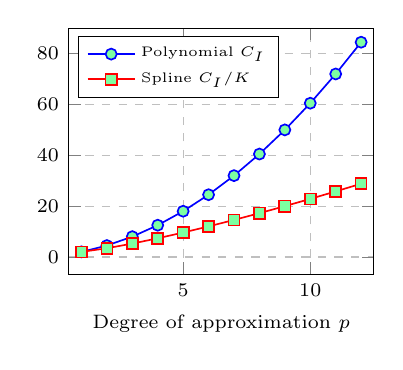
\begin{tikzpicture}
\begin{axis}[
width=.45\textwidth,
    xlabel={Degree of approximation $p$},   
%    ylabel={$C_I / K$},
    xmin=.5, xmax=12.5,
    ymax=0,ymax=90,    
    legend pos=north west, legend cell align=left, legend style={font=\tiny},	
    xmajorgrids=true,  ymajorgrids=true, grid style=dashed,
] 

\addplot[color=blue,mark=*,semithick, mark options={fill=markercolor}]
coordinates{(1,2)(2,4.5)(3,8)(4,12.5)(5,18)(6,24.5)(7,32)(8,40.5)(9,50)(10,60.5)(11,72)(12,84.5)};
\addplot[color=red,mark=square*,semithick, mark options={fill=markercolor}]
coordinates{(1,2)(2,3.42857)(3,5.27022)(4,7.3491)(5,9.61122)(6,12.0258)(7,14.5716)(8,17.233)(9,19.9977)(10,22.8559)(11,25.7995)(12,28.8217)};
%\addplot[color=black,mark=triangle*,semithick, mark options={fill=markercolor}]
%coordinates{(1,2)(2,3.15356)(3,4.41024)(4,5.72791)(5,7.09105)(6,8.48919)(7,9.91299)(8,11.3583)(9,12.8221)(10,14.3019)(11,15.796)(12,17.3028)};

\legend{Polynomial $C_I$, Spline $C_I/K$}%, Smoothed $C_I/K$ }
\end{axis}
\end{tikzpicture}
}
\hspace{1em}
\subfloat[Trace constants, $K = 2p$]{
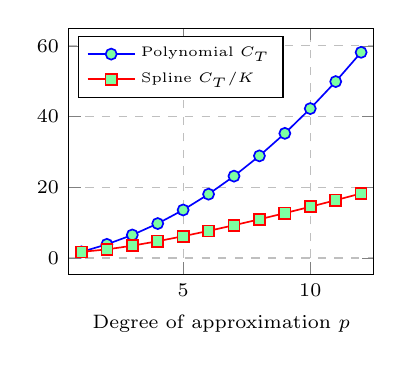
\begin{tikzpicture}
\begin{axis}[
width=.45\textwidth,
    xlabel={Degree of approximation $p$},   
    xmin=.5, xmax=12.5,
    ymax=0,ymax=65,    
    legend pos=north west, legend cell align=left, legend style={font=\tiny},	
    xmajorgrids=true,  ymajorgrids=true, grid style=dashed,
] 

\addplot[color=blue,mark=*,semithick, mark options={fill=markercolor}]
coordinates{(1,1.73205)(2,3.87298)(3,6.5216)(4,9.74981)(5,13.5914)(6,18.0596)(7,23.1598)(8,28.894)(9,35.2634)(10,42.2685)(11,49.9096)(12,58.187)};
\addplot[color=red,mark=square*,semithick, mark options={fill=markercolor}]
coordinates{(1,1.73205)(2,2.43668)(3,3.48657)(4,4.75661)(5,6.16327)(6,7.6751)(7,9.27477)(8,10.9506)(9,12.694)(10,14.4983)(11,16.3578)(12,18.2682)};
%\addplot[color=black,mark=triangle*,semithick, mark options={fill=markercolor}]
%coordinates{(1,1.73205)(2,2.32019)(3,2.9916)(4,3.77273)(5,4.61001)(6,5.4806)(7,6.37331)(8,7.28317)(9,8.20701)(10,9.14265)(11,10.0885)(12,11.0432)};

\legend{Polynomial $C_T$, Spline $C_T/K$}%, Smoothed $C_T/K$ }
\end{axis}
\end{tikzpicture}
}
\caption*{Polynomial constants are $O(p^2)$, observed spline constants \textcolor{red}{$O(p)$} for $K \geq O(1/p)$.}
\let\thefootnote\relax\footnotetext{\tiny Takacs, Takacs (2016). \textit{Approximation error estimates and inverse inequalities for B-splines of maximum smoothness}.}
}
\end{figure}
\only<2->{\uncover<3->{
\begin{center}
\ovalbox{\textcolor{red}{$dt \propto \frac{h}{p^2}$} for $C^0$-FEM and DG, \textcolor{red}{$dt \propto \frac{h}{p}$} for IGA!}
\end{center}}}
}

\section{Optimizing splines for explicit solvers}
\frame[noframenumbering]{
\tableofcontents[currentsection]
}

\frame{
\frametitle{B-spline bases and optimal spline spaces}
\vspace{-1em}
\begin{figure}
\centering
\subfloat[Uniform knots]{\includegraphics[width=.32\textwidth]{figs/unifknots.png}}
\hspace{2.5em}
\subfloat[Optimal knots]{\includegraphics[width=.32\textwidth]{figs/optknots.png}}
%\caption{B-spline bases with uniform and optimal knot vectors ($p = 4, K = 4$).}
\end{figure}

\begin{itemize}
\item Sup-inf: ``worst best approximation'' in $X$ from $X_n$ 
\[
d_n(X;X_n) =  \sup_{x\in X} \inf_{y\in X_n} \nor{x - y}, \qquad {\rm dim}\LRp{X_n} = n.
\]
\item Spline spaces with optimal knot vectors: minimal sup-inf for
\[
X = \LRc{f \in L^2([-1,1]): \pd{f}{x}{p-1} \text{ continuous}, \quad \nor{f}_{L^2} \leq 1},
\]
\end{itemize}

\let\thefootnote\relax\footnotetext{\tiny Melkman and Micchelli (1978). \textit{Spline spaces are optimal for $L^2$ $n$-width}.}
}

\frame{
\frametitle{Optimal knot vectors: roots of eigenfunctions}
\setcounter{subfigure}{0}
\vspace{-1em}
\begin{figure}
\centering
\subfloat[$p = 2$]{\includegraphics[width=.33\textwidth]{figs/fnwidth_N2_K8.png}}
\subfloat[$p = 3$]{\includegraphics[width=.33\textwidth]{figs/fnwidth_N3_K8.png}}
\subfloat[$p = 4$]{\includegraphics[width=.33\textwidth]{figs/fnwidth_N4_K8.png}}
\caption{Eigenfunctions $y_{K+1,p}(x)$ for $K=8$ and various $p$.}
\end{figure}
\vspace{-1em}
\begin{itemize}
\item Optimal knots are roots of eigenfunctions $y_{K+1,p}(x)$.
\[
(-1)^p \frac{\partial^{2p}y}{\partial x^{2p}} = \lambda y(x), \qquad \frac{\partial^k y}{\partial x^k}(-1) = \frac{\partial^k y}{\partial x^k}(1) = 0, \quad 1\leq k \leq p-1.
\]
\item Approximate $y_{K+1,p}(x)$ using fine spline space; difficult for high $K, p$!
\end{itemize}
}

\frame{
\frametitle{Knot smoothing: approximating optimal knots}
\vspace{-.25em}
\begin{figure}
\begin{overlayarea}{\textwidth}{.5\textheight}
\centering
\only<1-2>{
\setcounter{subfigure}{0}
\subfloat[Knots $\xi_i$ (optimal in red)]{\includegraphics[width=.375\textwidth]{figs/knots.png}}
\hspace{2em}
\subfloat[Greville abscissae $\tau_j$]{\includegraphics[width=.375\textwidth]{figs/greville.png}}
}
%\only<3>{
%\setcounter{subfigure}{0}
%\subfloat{
%\begin{tikzpicture}
%\begin{axis}[
%width=.425\textwidth,
%    xlabel={Number of elements $K$},   
%        ylabel={Max knot error},
%    xmin=2, xmax=66,
%    ymax=0,ymax=0.0125,    
%    legend pos=north east, legend cell align=left, legend style={font=\tiny},	
%       xmajorgrids=true,  ymajorgrids=true, grid style=dashed,
%] 
%
%\addplot[color=blue,mark=*,semithick, mark options={fill=markercolor}]
%coordinates{(4,0.0121)(8,0.0075)(16,0.0046)(32,0.0023)(64,0.0012)};
%
%\addplot[color=red,mark=square*,semithick, mark options={fill=markercolor}]
%coordinates{(4,0.009)(8,0.0041)(16,0.0028)(32,0.002)(64,0.0012)};
%
%\addplot[color=black,mark=triangle*,semithick, mark options={fill=markercolor}]
%coordinates{(4,0.0016)(8,0.0101)(16,0.0074)(32,0.0048)(64,0.0028)};
%
%\legend{$p = 2$, $p=3$, $p=4$}
%\end{axis}
%\end{tikzpicture}
%}
%\hspace{2em}
%\subfloat{
%\begin{tikzpicture}
%\begin{axis}[
%width=.425\textwidth,
%    xlabel={Number of elements $K$},   
%    ylabel={Max Greville error},
%    xmin=2, xmax=66,
%    ymax=0,ymax=0.0125,    
%    legend pos=north east, legend cell align=left, legend style={font=\tiny},	
%       xmajorgrids=true,  ymajorgrids=true, grid style=dashed,
%] 
%
%\addplot[color=blue,mark=*,semithick, mark options={fill=markercolor}]
%coordinates{(4,0.006)(8,0.0038)(16,0.0024)(32,0.0011)(64,0.00058806)};
%
%\addplot[color=red,mark=square*,semithick, mark options={fill=markercolor}]
%coordinates{(4,0.003)(8,0.002)(16,0.0018)(32,0.0012)(64,0.00067857)};
%
%\addplot[color=black,mark=triangle*,semithick, mark options={fill=markercolor}]
%coordinates{(4,0.000401)(8,0.0025)(16,0.0016)(32,0.00089352)(64,0.00063901)};
%
%\legend{$p = 2$, $p=3$, $p=4$}
%\end{axis}
%\end{tikzpicture}
%}
%}
\end{overlayarea}
%\caption{Knot locations for iterations $k = 0, \ldots, 10$ for a spline space with $p = 3, K = 8$.  Computed optimal knot positions and Greville abscissae are overlaid in \textcolor{red}{red}.}
\label{fig:smoothedknots}
\end{figure}
\vspace{-1.25em}
\begin{itemize}
\item Greville abscissae $\tau_j$: coefficients for linear coordinate $x$.
\only<1>{
\[
x = \sum_{1\leq j \leq p+K} \tau_j B^p_j(x), \qquad \tau_j = \frac{1}{p}\sum_{1\leq i \leq p} \xi_{i+j-1}, \quad j = 1,\ldots,p.
\]  
}
\only<2->{
\[
\textcolor{red}{\xi_i} = \sum_{1\leq j \leq p+K} \tau_j B^p_j(\textcolor{red}{\xi_i}), \qquad \tau_j = \frac{1}{p}\sum_{1\leq i \leq p} \xi_{i+j-1}, \quad j = 1,\ldots,p.
\]  
}
\item Replace Greville abscissae with equispaced points $\widehat{x}_i$ and iterate 
\[
\tilde{\xi}^{k+1}_i = \sum_{1\leq j\leq p+K} \widehat{x}_i B^p_j(\xi_i;  \tilde{\xi}^k), \qquad \tilde{\xi}^0_i = \xi_i,
\]
\end{itemize}
}

\frame{
\frametitle{Approximation properties in 1D: oscillatory functions}
\setcounter{subfigure}{0}

\vspace{-1em}
\begin{figure}
\centering
\subfloat[First order formulation]{
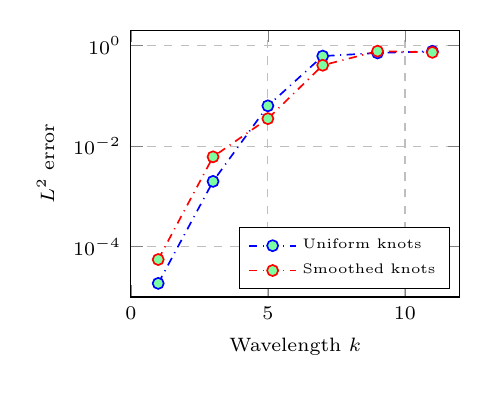
\begin{tikzpicture}
\begin{semilogyaxis}[
width=.475\textwidth,
    xlabel={Wavelength $k$},   
    ylabel={$L^2$ error},
    ymin=1e-5, ymax=2,    
    legend pos=south east, legend cell align=left, legend style={font=\tiny},	
       xmajorgrids=true,  ymajorgrids=true, grid style=dashed,
] 
\addplot[color=blue,mark=*, dashdotted, semithick, mark options={solid,fill=markercolor}]
coordinates{(1,1.86794e-05)(3,0.00199192)(5,0.0632619)(7,0.616786)(9,0.712371)(11,0.768705)};
\addplot[color=red,mark=*, dashdotted, semithick, mark options={solid,fill=markercolor}]
coordinates{(1,5.56475e-05)(3,0.00612773)(5,0.0351819)(7,0.405041)(9,0.772862)(11,0.731632)};
\legend{Uniform knots, Smoothed knots}
\end{semilogyaxis}
\end{tikzpicture}
}
\subfloat[Second order formulation]{
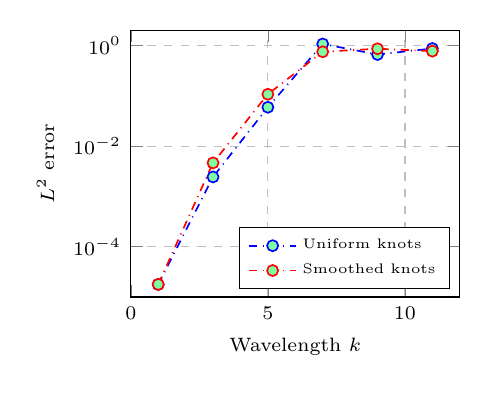
\begin{tikzpicture}
\begin{semilogyaxis}[
width=.475\textwidth,
    xlabel={Wavelength $k$},   
    ylabel={$L^2$ error},
    ymin=1e-5, ymax=2,    
    legend pos=south east, legend cell align=left, legend style={font=\tiny},	
       xmajorgrids=true,  ymajorgrids=true, grid style=dashed,
] 
\addplot[color=blue,mark=*, dashdotted, semithick, mark options={solid,fill=markercolor}]
coordinates{(1,1.77384e-05)(3,0.00244169)(5,0.0592546)(7,1.07406)(9,0.662767)(11,0.872701)};
\addplot[color=red,mark=*, dashdotted, semithick, mark options={solid,fill=markercolor}]
coordinates{(1,1.78285e-05)(3,0.00465007)(5,0.107561)(7,0.751711)(9,0.864029)(11,0.773654)};

\legend{Uniform knots, Smoothed knots}
\end{semilogyaxis}
\end{tikzpicture}
}
\caption{$L^2$ errors for 1D acoustics using uniform and smoothed knot vectors: smoothed knots emphasize high frequencies over low frequencies. }
\end{figure}
}


%\frame{
%\frametitle{Spectral properties of $\bm{A}_h$}
%\setcounter{subfigure}{0}
%\vspace{.5em}
%\only<2>{
%Constant 1D advection: numerical dispersion error $\LRb{{\rm Re}(\omega) - {\rm Re}(\omega_h)}$
%\[
%\pd{u}{t}{} + \pd{u}{x}{} = 0, \qquad u(x,t) = e^{i(kx - \omega t)}, \quad u_h(x,t) = e^{i(kx-\omega_h t)}.
%\]
%\vspace{-2em}
%\begin{figure}
%\centering
%\subfloat[Dispersion errors (uniform knots)]{
%\includegraphics[width=.45\textwidth]{figs/dispersionErrUnif.png}
%}
%\subfloat[Dispersion errors (smoothed knots)]{
%\includegraphics[width=.45\textwidth]{figs/dispersionErrSmooth.png}
%}
%\caption{Dispersion errors using full upwinding, $p = 4$, and $K = 1, 4, 8$. } %The exact dispersion relation is given as a black dotted line.}% in Figures~\ref{subfig:disp1}, \ref{subfig:disp2}.  }
%%\label{fig:eigerr1}
%\end{figure}
%
%}
%\only<1>{
%Eigenvalues, eigenfunctions of 1D Laplacian: uniform vs smoothed knots.
%\[
%\LRb{\lambda_k-\lambda_{h,k}}, \qquad \nor{w_k(x)-w_{h,k}(x)}_{L^2}^2
%\]
%\vspace{-1.5em}
%%\[
%%-\pd{u}{x}{2} = \lambda u, \qquad \LRp{\Grad u, \Grad v}_{\Omega} = \lambda_h \LRp{u,v}_{\Omega}, \quad \forall v\in V_h.
%%\]
%\begin{figure}
%\centering
%\subfloat[Eigenvalue errors]{
%\includegraphics[width=.45\textwidth]{figs/eigvals2ndorder.png}
%}
%\subfloat[Eigenvector errors]{
%\includegraphics[width=.45\textwidth]{figs/eigfunc2ndorder.png}
%}
%\caption{Eigenvalue and eigenvector errors for $p = 4, K = 32$ splines. }
%\end{figure}
%}
%}


\frame{
\frametitle{Approximation properties in 2D/3D: curvilinear domains}

\begin{overlayarea}{\textwidth}{\textheight}

\begin{itemize}
\item<1-> Smoothed knot vectors: more accurate on curved domains.
\item<2-> Differences between first, second order forms ($L^2$ vs energy norm?).
\end{itemize}
\vspace{-1.5em}
%\begin{overlayarea}{\textwidth}{.725\textheight}
\only<1>{
\begin{figure}
\centering
\subfloat[Warped mesh, $\alpha = 1/8$]{\includegraphics[width=.375\textwidth]{figs/mapped.png}}
\subfloat[$L^2$ errors ($\alpha = 1/64$) ]{
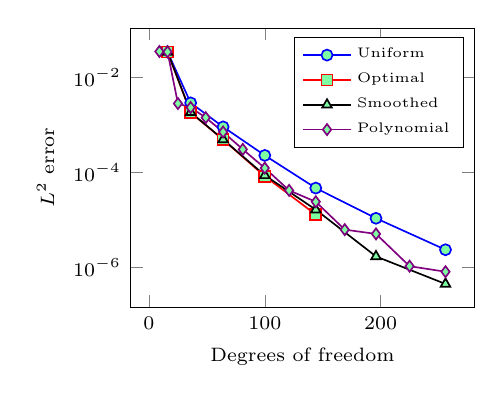
\begin{tikzpicture}
\begin{semilogyaxis}[
    legend cell align=left,
    legend style={legend pos=north east, font=\tiny},
    width=.49\textwidth,
    xlabel={Degrees of freedom},
    ylabel={$L^2$ error}, 
    grid style=dashed,
] 
\addplot[color=blue,mark=*,semithick, mark options={solid,fill=markercolor}]
coordinates{(16,0.0345598)(36,0.00291687)(64,0.000910808)(100,0.000228283)(144,4.68154e-05)(196,1.08049e-05)(256,2.35056e-06)};
%[yshift=4pt] node[above, pos=.8, color=black] {$\alpha = 1/64$};
\addplot[color=red,mark=square*,semithick, mark options={solid,fill=markercolor}]
coordinates{(16,0.0345598)(36,0.0018151)(64,0.000489718)(100,8.29769e-05)(144,1.29416e-05)};
\addplot[color=black,mark=triangle*,semithick, mark options={solid,fill=markercolor}]
coordinates{(16,0.0345598)(36,0.00184734)(64,0.000495297)(100,8.68887e-05)(144,1.63983e-05)(196,1.69855e-06)(256,4.46827e-07)};
\addplot[color=violet,mark=diamond*,semithick, mark options={solid,fill=markercolor}]
coordinates{(9,0.0353096)(16,0.0346236)(25,0.00282808)(36,0.00233183)(49,0.00142429)(64,0.000710684)(81,0.000305903)(100,0.000123394)(121,4.1829e-05)(144,2.40683e-05)(169,6.2327e-06)(196,5.06423e-06)(225,1.05795e-06)(256,8.08652e-07)};
\legend{Uniform, Optimal, Smoothed, Polynomial}
%\legend{Uniform, Optimal, Smoothed}
\end{semilogyaxis}
\end{tikzpicture}
}
\caption{$L^2$ approx.\ errors: $\cos\LRp{\frac{\pi x}{2}}\cos\LRp{\frac{\pi y}{2}}$, $p = 2,\ldots, 8$ and $K = p$. }
\end{figure}
}


\only<2>{
\vspace{.5em}
\begin{figure}
\centering
\subfloat[First order formulation]{
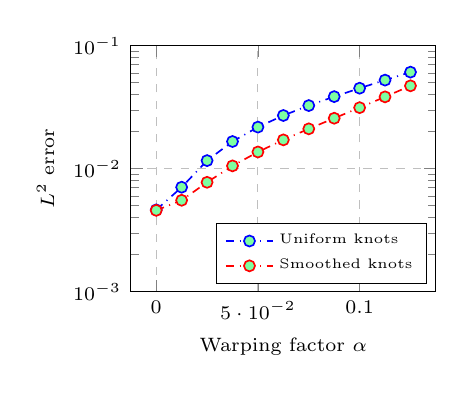
\begin{tikzpicture}
\begin{semilogyaxis}[
width=.45\textwidth,
    xlabel={Warping factor $\alpha$},   
    ylabel={$L^2$ error},
    ymin=1e-3, ymax=.1,    
    legend pos=south east, legend cell align=left, legend style={font=\tiny},	
       xmajorgrids=true,  ymajorgrids=true, grid style=dashed,
] 
\addplot[color=blue,mark=*, dashdotted, semithick, mark options={solid,fill=markercolor}]
coordinates{(0,0.00462693)(0.0125,0.007073)(0.025,0.0116375)(0.0375,0.0166377)(0.05,0.021786)(0.0625,0.0270765)(0.075,0.0326103)(0.0875,0.0385547)(0.1,0.0451154)(0.1125,0.0525108)(0.125,0.0609548)};
\addplot[color=red,mark=*, dashdotted, semithick, mark options={solid,fill=markercolor}]
coordinates{(0,0.00458676)(0.0125,0.0055373)(0.025,0.00775311)(0.0375,0.0105429)(0.05,0.0136791)(0.0625,0.0171546)(0.075,0.0210896)(0.0875,0.0257146)(0.1,0.0313525)(0.1125,0.0383814)(0.125,0.0471834)};

\legend{Uniform knots, Smoothed knots}
\end{semilogyaxis}
\end{tikzpicture}
}
\subfloat[Second order formulation]{
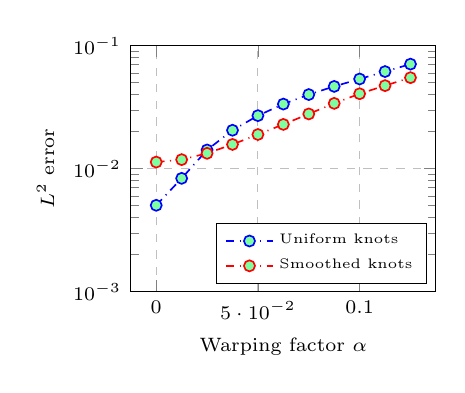
\begin{tikzpicture}
\begin{semilogyaxis}[
width=.45\textwidth,
    xlabel={Warping factor $\alpha$},   
    ylabel={$L^2$ error},
    ymin=1e-3, ymax=.1,    
    legend pos=south east, legend cell align=left, legend style={font=\tiny},	
       xmajorgrids=true,  ymajorgrids=true, grid style=dashed,
] 
\addplot[color=blue,mark=*, dashdotted, semithick, mark options={solid,fill=markercolor}]
coordinates{(0,0.00504237)(0.0125,0.00834838)(0.025,0.0142055)(0.0375,0.0205381)(0.05,0.0269995)(0.0625,0.0335261)(0.075,0.0400686)(0.0875,0.0466709)(0.1,0.0536183)(0.1125,0.0616203)(0.125,0.0708213)};
\addplot[color=red,mark=*, dashdotted, semithick, mark options={solid,fill=markercolor}]
coordinates{(0,0.0113237)(0.0125,0.0118539)(0.025,0.013336)(0.0375,0.0157542)(0.05,0.0189697)(0.0625,0.0229092)(0.075,0.027875)(0.0875,0.0339693)(0.1,0.0406825)(0.1125,0.0473484)(0.125,0.0549665)};

\legend{Uniform knots, Smoothed knots}
\end{semilogyaxis}
\end{tikzpicture}
}
\caption{$L^2$ errors  w.r.t.\ curved warping for 2D acoustics ($p = 3, K= 8$ splines).}
\label{fig:warpingconverge}
\end{figure}
}
\end{overlayarea}
}

\frame{
\frametitle{Smoothed knot vectors improve the CFL}

\begin{figure}
\centering
\only<1>{
\setcounter{subfigure}{0}
\subfloat[Inverse constants, $K = 2p$]{
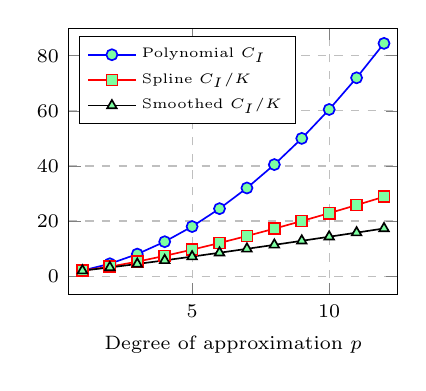
\begin{tikzpicture}
\begin{axis}[
width=.475\textwidth,
    xlabel={Degree of approximation $p$},   
%    ylabel={$C_I / K$},
    xmin=.5, xmax=12.5,
    ymax=0,ymax=90,    
    legend pos=north west, legend cell align=left, legend style={font=\tiny},	
    xmajorgrids=true,  ymajorgrids=true, grid style=dashed,
] 

\addplot[color=blue,mark=*,semithick, mark options={fill=markercolor}]
coordinates{(1,2)(2,4.5)(3,8)(4,12.5)(5,18)(6,24.5)(7,32)(8,40.5)(9,50)(10,60.5)(11,72)(12,84.5)};
\addplot[color=red,mark=square*,semithick, mark options={fill=markercolor}]
coordinates{(1,2)(2,3.42857)(3,5.27022)(4,7.3491)(5,9.61122)(6,12.0258)(7,14.5716)(8,17.233)(9,19.9977)(10,22.8559)(11,25.7995)(12,28.8217)};
\addplot[color=black,mark=triangle*,semithick, mark options={fill=markercolor}]
coordinates{(1,2)(2,3.15356)(3,4.41024)(4,5.72791)(5,7.09105)(6,8.48919)(7,9.91299)(8,11.3583)(9,12.8221)(10,14.3019)(11,15.796)(12,17.3028)};

\legend{Polynomial $C_I$, Spline $C_I/K$, Smoothed $C_I/K$ }
\end{axis}
\end{tikzpicture}
}
\hspace{1em}
\subfloat[Trace constants, $K = 2p$]{
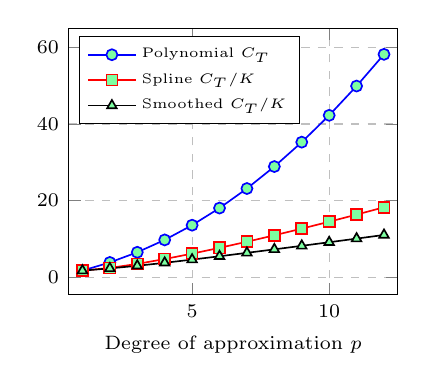
\begin{tikzpicture}
\begin{axis}[
width=.475\textwidth,
    xlabel={Degree of approximation $p$},   
    xmin=.5, xmax=12.5,
    ymax=0,ymax=65,    
    legend pos=north west, legend cell align=left, legend style={font=\tiny},	
    xmajorgrids=true,  ymajorgrids=true, grid style=dashed,
] 

\addplot[color=blue,mark=*,semithick, mark options={fill=markercolor}]
coordinates{(1,1.73205)(2,3.87298)(3,6.5216)(4,9.74981)(5,13.5914)(6,18.0596)(7,23.1598)(8,28.894)(9,35.2634)(10,42.2685)(11,49.9096)(12,58.187)};
\addplot[color=red,mark=square*,semithick, mark options={fill=markercolor}]
coordinates{(1,1.73205)(2,2.43668)(3,3.48657)(4,4.75661)(5,6.16327)(6,7.6751)(7,9.27477)(8,10.9506)(9,12.694)(10,14.4983)(11,16.3578)(12,18.2682)};
\addplot[color=black,mark=triangle*,semithick, mark options={fill=markercolor}]
coordinates{(1,1.73205)(2,2.32019)(3,2.9916)(4,3.77273)(5,4.61001)(6,5.4806)(7,6.37331)(8,7.28317)(9,8.20701)(10,9.14265)(11,10.0885)(12,11.0432)};

\legend{Polynomial $C_T$, Spline $C_T/K$, Smoothed $C_T/K$ }
\end{axis}
\end{tikzpicture}}
\caption{Knot smoothing results in roughly $2\times$ smaller trace, inverse constants.}
}
\only<2>{
\setcounter{subfigure}{0}
\subfloat[Uniform knots]{
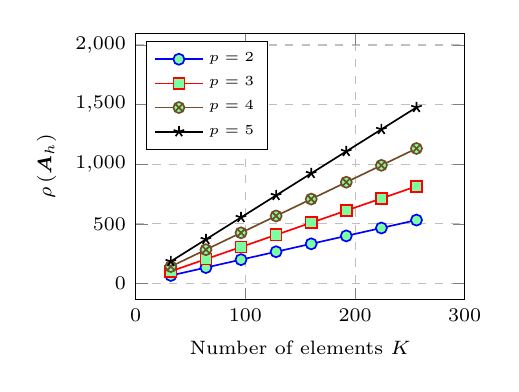
\begin{tikzpicture}
\begin{axis}[
width=.475\textwidth,
    xlabel={Number of elements $K$},   
    ylabel={$\rho\LRp{\bm{A}_h}$},       
    xmin=0, xmax=300,
    ymax=0,ymax=2100,    
    legend pos=north west, legend cell align=left, legend style={font=\tiny},	
       xmajorgrids=true,  ymajorgrids=true, grid style=dashed,
] 
\addplot+[semithick, mark options={solid,fill=markercolor}]
coordinates{(32,66.4194)(64,132.839)(96,199.258)(128,265.678)(160,332.097)(192,398.517)(224,464.936)(256,531.355)};
\addplot+[semithick, mark options={solid,fill=markercolor}]
coordinates{(32,101.838)(64,203.677)(96,305.515)(128,407.354)(160,509.192)(192,611.031)(224,712.869)(256,814.707)};
\addplot+[semithick, mark options={solid,fill=markercolor}]
coordinates{(32,141.497)(64,282.993)(96,424.49)(128,565.987)(160,707.484)(192,848.98)(224,990.477)(256,1131.97)};
\addplot+[semithick, mark options={solid,fill=markercolor}]
coordinates{(32,184.614)(64,369.228)(96,553.842)(128,738.456)(160,923.07)(192,1107.68)(224,1292.3)(256,1476.91)};


\legend{$p = 2$, $p=3$, $p=4$, $p = 5$}
\end{axis}
\end{tikzpicture}
}
\subfloat[Smoothed knots]{
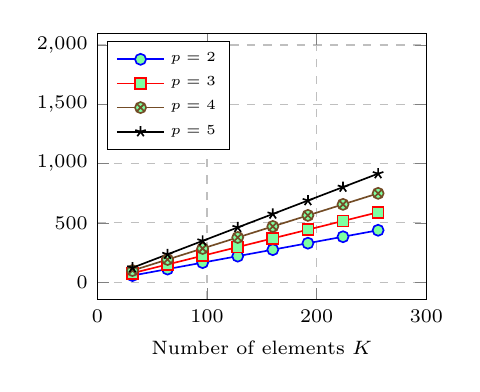
\begin{tikzpicture}
\begin{axis}[
width=.475\textwidth,
    xlabel={Number of elements $K$},   
%    ylabel={$\rho\LRp{\bm{A}_h}$},   
    xmin=0, xmax=300,
    ymax=0,ymax=2100,    
    legend pos=north west, legend cell align=left, legend style={font=\tiny},	
       xmajorgrids=true,  ymajorgrids=true, grid style=dashed,
] 

\addplot+[semithick, mark options={solid,fill=markercolor}]
coordinates{(32,55.5039)(64,110.088)(96,164.669)(128,219.248)(160,273.827)(192,328.405)(224,382.984)(256,437.563)};
\addplot+[semithick, mark options={solid,fill=markercolor}]
coordinates{(32,75.8822)(64,149.237)(96,222.58)(128,295.92)(160,369.26)(192,442.599)(224,515.938)(256,589.276)};
\addplot+[semithick, mark options={solid,fill=markercolor}]
coordinates{(32,97.8724)(64,190.915)(96,283.926)(128,376.931)(160,469.932)(192,562.932)(224,655.931)(256,748.929)};
\addplot+[semithick, mark options={solid,fill=markercolor}]
coordinates{(32,121.298)(64,234.744)(96,348.126)(128,461.491)(160,574.85)(192,688.206)(224,801.56)(256,914.912)};

\legend{$p = 2$, $p=3$, $p=4$, $p = 5$}
\end{axis}
\end{tikzpicture}
}
\caption{Growth of $\rho\LRp{\bm{A}_h}$ for advection using spline spaces of degree $p = 2, \ldots, 5$. }
}
\only<3>{
\setcounter{subfigure}{0}
\subfloat[Uniform knots]{
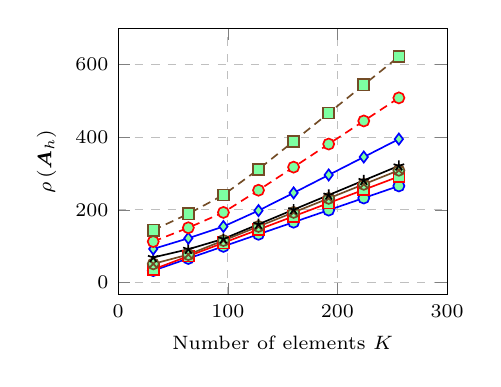
\begin{tikzpicture}
\begin{axis}[
width=.475\textwidth,
    xlabel={Number of elements $K$},   
        ylabel={$\rho\LRp{\bm{A}_h}$},       
    xmin=0, xmax=300,
    ymax=0,ymax=700,    
    legend pos=north west, legend cell align=left, legend style={font=\tiny},	
       xmajorgrids=true,  ymajorgrids=true, grid style=dashed,
] 
\addplot+[semithick, mark options={solid,fill=markercolor}]
coordinates{(32,32.9239)(64,66.339)(96,99.6489)(128,132.926)(160,166.191)(192,199.449)(224,232.703)(256,265.956)};
\addplot+[semithick, mark options={solid,fill=markercolor}]
coordinates{(32,36.0829)(64,72.8362)(96,109.357)(128,145.911)(160,182.425)(192,218.937)(224,255.45)(256,291.953)};
\addplot+[semithick, mark options={solid,fill=markercolor}]
coordinates{(32,51.525)(64,77.0896)(96,115.797)(128,154.475)(160,193.14)(192,231.798)(224,270.454)(256,309.109)};
\addplot+[semithick, mark options={solid,fill=markercolor}]
coordinates{(32,69.1513)(64,91.7232)(96,120.356)(128,160.533)(160,200.771)(192,240.95)(224,281.151)(256,321.333)};
\addplot+[semithick, mark options={solid,fill=markercolor}]
coordinates{(32,92.592)(64,121.947)(96,154.335)(128,198.112)(160,246.867)(192,296.187)(224,345.548)(256,394.912)};
\addplot+[semithick, mark options={solid,fill=markercolor}]
coordinates{(32,112.952)(64,150.924)(96,193.087)(128,254.178)(160,317.703)(192,381.243)(224,444.784)(256,508.325)};
\addplot+[semithick, mark options={solid,fill=markercolor}]
coordinates{(32,144.171)(64,189.195)(96,241.188)(128,311.773)(160,388.78)(192,466.469)(224,544.209)(256,621.953)};

%\addplot[color=black,dashed,semithick, mark options={solid,fill=markercolor}]
%coordinates{(32,32)(64,64)(96,96)(128,128)(160,160)(192,192)(224,224)(256,256)}; % O(2/h) line
%\legend{$p = 2$, $p=3$, $p=4$, $p = 5$, $p = 6$, $p = 7$, $p=8$}
%\legend{$\frac{1}{h}$, $\frac{1.5}{h}$}
\end{axis}
\end{tikzpicture}
}
\subfloat[Smoothed knots]{
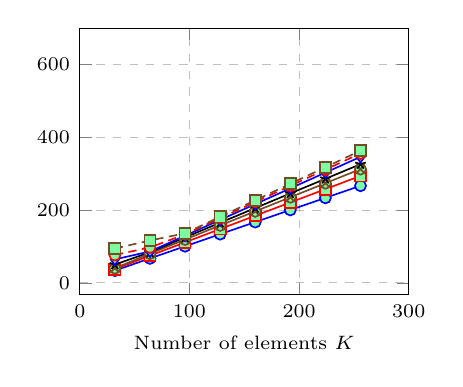
\begin{tikzpicture}
\begin{axis}[
width=.475\textwidth,
    xlabel={Number of elements $K$},   
%        ylabel={$\rho\LRp{\bm{A}_h}$},       
    xmin=0, xmax=300,
    ymax=0,ymax=700,    
    legend pos=north west, legend cell align=left, legend style={font=\tiny},	
       xmajorgrids=true,  ymajorgrids=true, grid style=dashed,
] 

%\addplot[color=black,semithick, mark options={solid,fill=markercolor}]
%coordinates{(32,32)(64,64)(96,96)(128,128)(160,160)(192,192)(224,224)(256,256)};% [yshift=-3pt] node[below, pos=.95,color=black] {$y = 1/h$};% O(1/h) line
%\addplot[color=red,semithick, mark options={solid,fill=markercolor}]
%coordinates{(32,48)(64,96)(96,144)(128,192)(160,240)(192,288)(224,336)(256,384)}; %[yshift=3pt] node[above, pos=.95,color=black] {$y = 1.5/h$};
%\pgfplotsset{cycle list set=0}
\addplot+[semithick, mark options={solid,fill=markercolor}]
coordinates{(32,33.8023)(64,67.3347)(96,100.665)(128,133.949)(160,167.218)(192,200.479)(224,233.737)(256,266.992)}; %p = 2
\addplot+[semithick, mark options={solid,fill=markercolor}]
coordinates{(32,37.5425)(64,74.8178)(96,111.545)(128,148.129)(160,184.671)(192,221.196)(224,257.712)(256,294.223)}; % p = 3
\addplot+[semithick, mark options={solid,fill=markercolor}]
coordinates{(32,40.4264)(64,80.3236)(96,119.264)(128,158.017)(160,196.716)(192,235.393)(224,274.059)(256,312.72)}; % p = 4
\addplot+[semithick, mark options={solid,fill=markercolor}]
coordinates{(32,50.3593)(64,84.3661)(96,125.088)(128,165.445)(160,205.705)(192,245.927)(224,286.133)(256,326.328)}; % p = 5
\addplot+[semithick, mark options={solid,fill=markercolor}]
coordinates{(32,64.6167)(64,86.4858)(96,129.798)(128,173.13)(160,216.469)(192,259.811)(224,303.155)(256,346.5)}; % p = 6
\addplot+[semithick, mark options={solid,fill=markercolor}]
coordinates{(32,76.7086)(64,97.5475)(96,133.384)(128,177.856)(160,222.354)(192,266.858)(224,311.365)(256,355.876)}; %p = 7
\addplot+[semithick, mark options={solid,fill=markercolor}]
coordinates{(32,94.4519)(64,116.577)(96,136.311)(128,181.68)(160,227.101)(192,272.535)(224,317.975)(256,363.42)};  % p =8
%\addplot[color=black,dashed,semithick, mark options={solid,fill=markercolor}]
%coordinates{(32,32)(64,64)(96,96)(128,128)(160,160)(192,192)(224,224)(256,256)}; % O(2/h) line
%\legend{$p = 2$, $p=3$, $p=4$, $p = 5$, $p = 6$, $p = 7$, $p=8$}
%\legend{${1}/{h}$, ${1.5}/{h}$}
\end{axis}
\end{tikzpicture}
}
\caption{Growth of $\rho\LRp{\bm{A}_h}$ using an \textcolor{red}{upwind flux} and spline spaces of degree $p = 2, \ldots, 8$.  \textcolor{red}{Nearly $p$-independent CFL observed for advection, acoustics}.}
}
\end{figure}
}


%\section{Numerical experiments}
%\frame[noframenumbering]{
%\frametitle{Outline}
%\tableofcontents[currentsection]
%}
%

\frame{
\frametitle{Acoustics: a 3D multi-patch example}
\setcounter{subfigure}{0}
\vspace{-1em}
\begin{figure}
\centering
\subfloat{
\includegraphics[width=.285\textwidth]{figs/pipe_crop.png}
}
\subfloat{
\includegraphics[width=.285\textwidth]{figs/pipeDG_crop.png}
}
\subfloat{
\includegraphics[width=.375\textwidth]{figs/pipeDG_cut.png}
}
%\caption{Multi-patch 3D pipe, .}
\vspace{1em}
\end{figure}
\begin{itemize}
\item 12 patch pipe model, first order formulation, pulse inflow condition.  
\vspace{.5em}
\item Isotropic $p=6, K=16$ splines, smoothed knots on each patch.
\end{itemize}
%\let\thefootnote\relax\footnotetext{\tiny Chan, Evans.\ 2017.  {Multi-patch discontinuous Galerkin spline FEM for time-domain wave propagation} (in preparation).}
}


\frame{
\frametitle{Summary and acknowledgements}

\begin{itemize}
\item Weight-adjusted mass matrix: restore Kronecker structure while retaining energy stability and high order accuracy.  
\vspace{.25em}
\item Improved $O(h/p)$ CFL scaling for IGA, optimal $L^2$ convergence rates.  
\vspace{.25em}
\item Smoothed knots: improved CFL, better curved approximations.
\vspace{.25em}
\item Future directions: curl-conforming spline spaces (Maxwells).
\vspace{.25em}
\item This research is supported by DMS-1719818 and DMS-1712639.  
\end{itemize}
\vspace{.5em}
\begin{center}
Thank you!  Questions?
\vspace{.25em}

{\includegraphics[width=.15\textwidth]{figs/nsf.jpg}}
\end{center}

\let\thefootnote\relax\footnotetext{\tiny Chan, Evans (2018). \textit{Multi-patch discontinuous Galerkin isogeometric analysis for wave propagation: explicit time-stepping and efficient mass matrix inversion}.}
%\let\thefootnote\relax\footnotetext{\tiny Chan, et al.\ 2016.  {Weight-adjusted DG methods: curvilinear meshes} (arXiv).  }
%\let\thefootnote\relax\footnotetext{\tiny Chan 2017.  Weight-adjusted DG methods: matrix-valued weights and elastic wave prop.\ in heterogeneous media (arXiv).}
%\let\thefootnote\relax\footnotetext{\tiny Chan, Warburton 2015. {GPU-accelerated Bernstein-Bezier DG methods for wave problems} (SISC).}
}

%\frame{
%\begin{center}
%The authors thank TOTAL E\&P Research and Technology USA\\
%for their generous support of this work.
%\end{center}
%\let\thefootnote\relax\footnotetext{\tiny Chan, Warburton 2015. {GPU-accelerated Bernstein-Bezier DG methods for wave problems}.}
%\let\thefootnote\relax\footnotetext{\tiny Chan, Warburton 2015.  A short note on a Bernstein-Bezier basis for the pyramid.  (SISC, accepted)}
%\let\thefootnote\relax\footnotetext{\tiny Chan, et al.\ 2016.  {WADG methods I: wave propagation in heterogeneous media}.  In preparation.}
%\let\thefootnote\relax\footnotetext{\tiny Chan, et al.\ 2016.  {WADG methods II: curvilinear meshes}.  In preparation.}
%}
%% =================== extra slides =======================

\begin{frame}[noframenumbering]
\frametitle{Additional slides }
\end{frame}

\frame[noframenumbering]{
\frametitle{Patch refinement vs knot insertion (uniform knots)}
\setcounter{subfigure}{0}
\begin{itemize}
\item Patch size $H$, number of sub-elements $K$: $h = H/K$.
\vspace{.125em}
\item Optimal $O(h^{p+1})$ $L^2$ error for both patch refinement, knot insertion.
%\item Time integration: low storage 5-stage 4th order Runge-Kutta. 
\end{itemize}
\vspace{-1em}
\begin{figure}
\centering
\subfloat[First order (uniform knots)]{
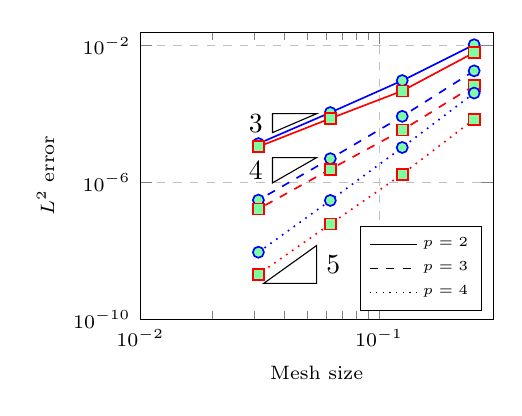
\begin{tikzpicture}
\begin{loglogaxis}[
width=.5\textwidth,
    xlabel={Mesh size },
    ylabel={$L^2$ error},
    xmin=1e-2, xmax=.3,
    ymin=1e-10, ymax=.025,    
    legend pos=south east, legend cell align=left, legend style={font=\tiny},	
       xmajorgrids=true,  ymajorgrids=true, grid style=dashed,
    legend entries={$p = 2$, $p=3$, $p=4$},
] 
\pgfplotsset{
cycle list={
{blue, mark=*}, {red,mark=square*},
{blue, mark=*,dashed}, {red,mark=square*,dashed},
{blue, mark=*,dotted}, {red,mark=square*,dotted},
legend style={mark options={no markers}}
}}
\addlegendimage{no markers,black}
\addlegendimage{no markers,black,dashed}
\addlegendimage{no markers,black,dotted}


\addplot+[semithick, mark options={solid,fill=markercolor}]
coordinates{(0.25,0.0106673)(0.125,0.000954815)(0.0625,0.000110851)(0.03125,1.37364e-05)};
\addplot+[semithick, mark options={solid,fill=markercolor}]
coordinates{(0.25,0.00629266)(0.125,0.000476247)(0.0625,7.45318e-05)(0.03125,1.11051e-05)};
\logLogSlopeTriangleFlip{.5}{.125}{.65}{3}{}

    % #1. Relative offset in x direction.
    % #2. Width in x direction, so xA-xB.
    % #3. Relative offset in y direction.
    % #4. Slope d(y)/d(log10(x)).

%    4.0252
\addplot+[semithick, mark options={solid,fill=markercolor}]
coordinates{(0.25,0.00183485)(0.125,8.58892e-05)(0.0625,4.97075e-06)(0.03125,3.0529e-07)};
%    3.8576
\addplot+[semithick, mark options={solid,fill=markercolor}]
coordinates{(0.25,0.000679534)(0.125,3.39478e-05)(0.0625,2.43527e-06)(0.03125,1.67989e-07)};
\logLogSlopeTriangleFlip{.5}{.125}{.475}{4}{}


%    5.0305
\addplot+[semithick, mark options={solid,fill=markercolor}]
coordinates{(0.25,0.000412175)(0.125,1.05591e-05)(0.0625,2.98645e-07)(0.03125,9.13748e-09)};
%    4.8741
\addplot+[semithick, mark options={solid,fill=markercolor}]
coordinates{(0.25,7.04497e-05)(0.125,1.74612e-06)(0.0625,6.0791e-08)(0.03125,2.07289e-09)};
\logLogSlopeTriangle{.5}{.15}{.125}{5}{}

\end{loglogaxis}
\end{tikzpicture}
}
\subfloat[Second order (uniform knots)]{
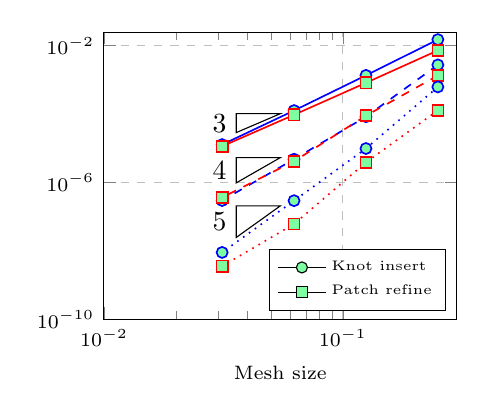
\begin{tikzpicture}
\begin{loglogaxis}[
width=.5\textwidth,
    xlabel={Mesh size}, 
%    ylabel={$L^2$ error},
    xmin=1e-2, xmax=.3,
    ymin=1e-10, ymax=.025,    
    legend pos=south east, legend cell align=left, legend style={font=\tiny},	
       xmajorgrids=true,  ymajorgrids=true, grid style=dashed,
%    legend entries={$p = 2$, $p=3$, $p=4$},
legend entries={Knot insert, Patch refine}
] 
\pgfplotsset{
cycle list={
{blue, mark=*}, {red,mark=square*},
{blue, mark=*,dashed}, {red,mark=square*,dashed},
{blue, mark=*,dotted}, {red,mark=square*,dotted},
legend style={mark options={no markers}}
}}
\addlegendimage{mark=*,black,mark options={solid,fill=markercolor}}
\addlegendimage{mark=square*,black,mark options={solid,fill=markercolor}}


\addplot+[semithick, mark options={solid,fill=markercolor}]
coordinates{(0.25,0.0150916)(0.125,0.00135624)(0.0625,0.000126749)(0.03125,1.27992e-05)};
\addplot+[semithick, mark options={solid,fill=markercolor}]
coordinates{(0.25,0.00727599)(0.125,0.000820116)(0.0625,9.52161e-05)(0.03125,1.14411e-05)};
\logLogSlopeTriangleFlip{.5}{.125}{.65}{3}{}

    % #1. Relative offset in x direction.
    % #2. Width in x direction, so xA-xB.
    % #3. Relative offset in y direction.
    % #4. Slope d(y)/d(log10(x)).

\addplot+[semithick, mark options={solid,fill=markercolor}]
coordinates{(0.25,0.00274207)(0.125,8.37621e-05)(0.0625,4.79288e-06)(0.03125,2.97136e-07)};
\addplot+[semithick, mark options={solid,fill=markercolor}]
coordinates{(0.25,0.001341)(0.125,8.99204e-05)(0.0625,4.17057e-06)(0.03125,3.6443e-07)};
\logLogSlopeTriangleFlip{.5}{.125}{.475}{4}{}

\addplot+[semithick, mark options={solid,fill=markercolor}]
coordinates{(0.25,0.000623337)(0.125,9.84177e-06)(0.0625,2.93926e-07)(0.03125,9.019e-09)};
\addplot+[semithick, mark options={solid,fill=markercolor}]
coordinates{(0.25,0.000128353)(0.125,3.87921e-06)(0.0625,6.10617e-08)(0.03125,3.57278e-09)};
\logLogSlopeTriangleFlip{.5}{.125}{.285}{5}{}

\end{loglogaxis}
\end{tikzpicture}
}
%\caption{Knot insertion vs patch refinement (uniform knots).  Results for knot insertion denoted by circles, results for patch refinement denoted by squares.}
\label{fig:hconvergence1D}
\end{figure}
}


\frame[noframenumbering]{
\frametitle{Behavior of weight-adjusted $L^2$ projection}

\only<1-3>{
Comparison with $L^2$ projection and Low-Storage Curvilinear DG
\[
\tilde{\phi}_i = \frac{\phi_i}{\sqrt{J}}, \qquad \bm{M}_{ij} = \int_{D^k} \tilde{\phi}_j\tilde{\phi}_i J = \int_{\widehat{D}} \phi_j\phi_i = \widehat{\bm{M}}_{ij}.
\]
\vspace{-2em}
}
\begin{figure}
\begin{overlayarea}{\textwidth}{.6\textheight}
\centering
\only<1>{
\subfloat{
\includegraphics[width=.37\textwidth]{figs/arnoldmesh1.png}
}
\subfloat{
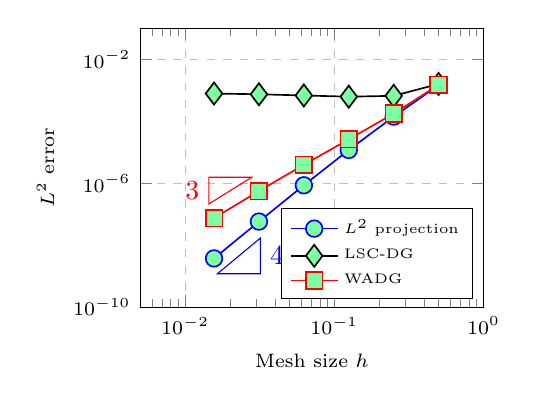
\begin{tikzpicture}
\begin{loglogaxis}[
	legend cell align=left,
	        legend style={font=\tiny},	
	width=.49\textwidth,
    xlabel={Mesh size $h$},
    ylabel={$L^2$ error},
    xmin=.005, xmax=1,
    ymin=1e-10, ymax=1e-1,
    legend pos=south east,
    xmajorgrids=true,
    ymajorgrids=true,
    grid style=dashed,
] 
% adding this 2x because pgfplots dashes the line for some reason...
\addplot[color=blue,mark=*,mark size=3,semithick, mark options={fill=markercolor}]
coordinates{(0.5,0.00145465)(0.25,0.000140693)(0.125,1.17949e-05)(0.0625,8.58138e-07)(0.03125,5.78543e-08)(0.015625,3.75483e-09)};
\addplot[color=black,mark=diamond*,mark size=4,semithick, mark options={fill=markercolor}]
coordinates{(0.5,0.00159198)(0.25,0.000658818)(0.125,0.000619747)(0.0625,0.000677173)(0.03125,0.00073964)(0.015625,0.000782687)};
\addplot[color=red,mark=square*,mark size=3,semithick, mark options={fill=markercolor}]
coordinates{(0.5,0.00148852)(0.25,0.000176325)(0.125,2.60169e-05)(0.0625,3.94602e-06)(0.03125,5.58752e-07)(0.015625,7.47639e-08)};
\logLogSlopeTriangleFlip{0.325}{0.125}{0.37}{3}{red};
\logLogSlopeTriangle{0.35}{0.125}{0.12}{4}{blue};

\legend{$L^2$ projection, LSC-DG, WADG}
\end{loglogaxis}
\end{tikzpicture}
}
\caption{Arnold-type mesh with $\nor{J}_{W^{N+1,\infty}} = O(h^{-1})$ for $N = 3$.}
}
\only<2>{
\subfloat{
\includegraphics[width=.37\textwidth]{figs/arnoldmesh2.png}
}
\subfloat{
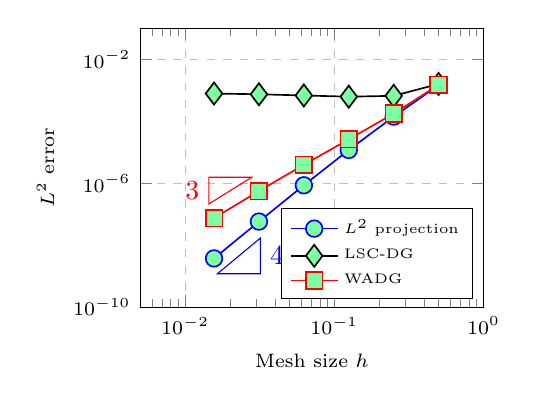
\begin{tikzpicture}
\begin{loglogaxis}[
	legend cell align=left,
	        legend style={font=\tiny},	
	width=.49\textwidth,
    xlabel={Mesh size $h$},
    ylabel={$L^2$ error},
    xmin=.005, xmax=1,
    ymin=1e-10, ymax=1e-1,
    legend pos=south east,
    xmajorgrids=true,
    ymajorgrids=true,
    grid style=dashed,
] 
% adding this 2x because pgfplots dashes the line for some reason...
\addplot[color=blue,mark=*,mark size=3,semithick, mark options={fill=markercolor}]
coordinates{(0.5,0.00145465)(0.25,0.000140693)(0.125,1.17949e-05)(0.0625,8.58138e-07)(0.03125,5.78543e-08)(0.015625,3.75483e-09)};
\addplot[color=black,mark=diamond*,mark size=4,semithick, mark options={fill=markercolor}]
coordinates{(0.5,0.00159198)(0.25,0.000658818)(0.125,0.000619747)(0.0625,0.000677173)(0.03125,0.00073964)(0.015625,0.000782687)};
\addplot[color=red,mark=square*,mark size=3,semithick, mark options={fill=markercolor}]
coordinates{(0.5,0.00148852)(0.25,0.000176325)(0.125,2.60169e-05)(0.0625,3.94602e-06)(0.03125,5.58752e-07)(0.015625,7.47639e-08)};
\logLogSlopeTriangleFlip{0.325}{0.125}{0.37}{3}{red};
\logLogSlopeTriangle{0.35}{0.125}{0.12}{4}{blue};

\legend{$L^2$ projection, LSC-DG, WADG}
\end{loglogaxis}
\end{tikzpicture}
}
\caption{Arnold-type mesh with $\nor{J}_{W^{N+1,\infty}} = O(h^{-1})$ for $N = 3$.}
}

\only<3>{
\subfloat{
\includegraphics[width=.37\textwidth]{figs/randunif1.png}
}
\subfloat{
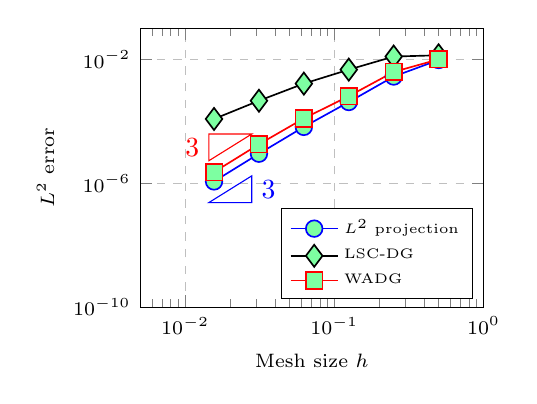
\begin{tikzpicture}
\begin{loglogaxis}[
	legend cell align=left,
	        legend style={font=\tiny},
	width=.49\textwidth,
    xlabel={Mesh size $h$},
    ylabel={$L^2$ error},
    xmin=.005, xmax=1,
    ymin=1e-10, ymax=1e-1,
    legend pos=south east,
    xmajorgrids=true,
    ymajorgrids=true,
    grid style=dashed,
] 
\addplot[color=blue,mark=*,mark size=3,semithick, mark options={fill=markercolor}]
coordinates{(0.5,0.00943375)(0.25,0.00276313)(0.125,0.000415615)(0.0625,6.56974e-05)(0.03125,8.95162e-06)(0.015625,1.14109e-06)};
\addplot[color=black,mark=diamond*,mark size=4,semithick, mark options={fill=markercolor}]
coordinates{(0.5,0.0134065)(0.25,0.012209)(0.125,0.004612)(0.0625,0.00163555)(0.03125,0.000458367)(0.015625,0.00011822)};
\addplot[color=red,mark=square*,mark size=3,semithick, mark options={fill=markercolor}]
coordinates{(0.5,0.00990795)(0.25,0.00389737)(0.125,0.00064227)(0.0625,0.000123078)(0.03125,1.80455e-05)(0.015625,2.28866e-06)};
\logLogSlopeTriangleFlip{0.325}{0.125}{0.525}{3}{red};
\logLogSlopeTriangle{0.325}{0.125}{0.375}{3}{blue};

\legend{$L^2$ projection, LSC-DG, WADG}
\end{loglogaxis}
\end{tikzpicture}
}
\caption{Curvilinear mesh constructed through random perturbation for $N = 3$.}
}
\only<4>{
\vspace{-2em}
High order convergence \textcolor{red}{slowed} by growth of $\nor{J}_{W^{N+1,\infty}} = O(h^N)$.
\vspace{1em}

\subfloat{
\includegraphics[width=.37\textwidth]{figs/curvarnold2ref.png}
}
\subfloat{
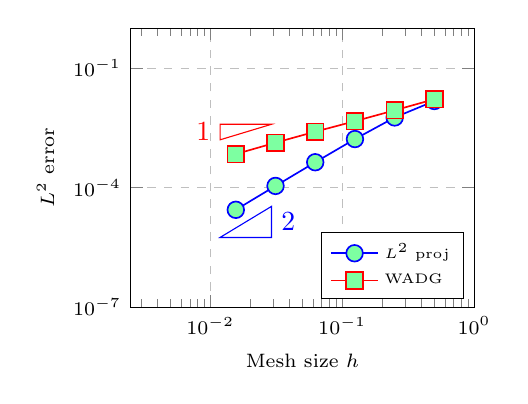
\begin{tikzpicture}
\begin{loglogaxis}[
legend style={font=\tiny},
	legend cell align=left,
	width=.49\textwidth,
    xlabel={Mesh size $h$},
    ylabel={$L^2$ error},
    xmin=.0025, xmax=1,
    ymin=1e-7, ymax=1e-0,
    legend pos=south east,
    xmajorgrids=true,
    ymajorgrids=true,
    grid style=dashed,
] 
% adding this 2x because pgfplots dashes the line for some reason...
\addplot[color=blue,mark=*,mark size=3,semithick, mark options={fill=markercolor}]
coordinates{(0.5,0.0149174)(0.25,0.00576658)(0.125,0.00165616)(0.0625,0.000433839)(0.03125,0.000110389)(0.015625,2.78024e-05)};
%\addplot[color=black,mark=diamond*,mark size=4,semithick, mark options={fill=markercolor}]
%coordinates{(0.5,0.018737)(0.25,0.0147278)(0.125,0.0117761)(0.0625,0.0110991)(0.03125,0.0112431)(0.015625,0.0114663)};
\addplot[color=red,mark=square*,mark size=3,semithick, mark options={fill=markercolor}]
coordinates{(0.5,0.0165783)(0.25,0.00872368)(0.125,0.00464969)(0.0625,0.00253621)(0.03125,0.00134518)(0.015625,0.000695124)};
\logLogSlopeTriangleFlip{0.41}{0.15}{0.6}{1}{red};
\logLogSlopeTriangle{0.41}{0.15}{0.25}{2}{blue};

%\node at (axis cs:.03,2.1e-07) {$a = 10^{-1}$};

%\legend{$L^2$ proj, LSC-DG, WADG}
\legend{$L^2$ proj, WADG}
\end{loglogaxis}
\end{tikzpicture}
}
\caption{Moderately warped curved Arnold-type mesh for $N = 3$.}
}
\only<5>{
\vspace{-2em}
High order convergence is \textcolor{red}{stalled} by growth of $\nor{J}_{W^{N+1,\infty}} = O(h^{N+1})$.  
\vspace{1em}

\subfloat{
\includegraphics[width=.37\textwidth]{figs/curvarnold1ref.png}
}
\subfloat{
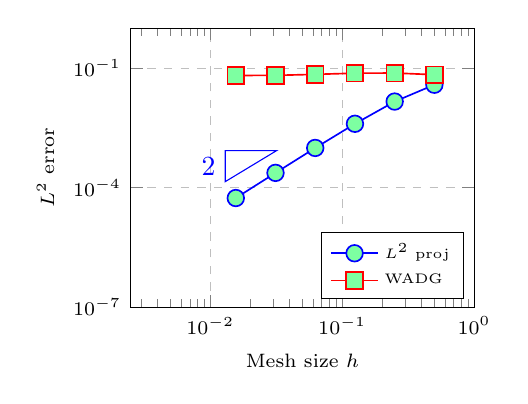
\begin{tikzpicture}
\begin{loglogaxis}[
legend style={font=\tiny},
	legend cell align=left,
	width=.49\textwidth,
    xlabel={Mesh size $h$},
    ylabel={$L^2$ error},
    xmin=.0025, xmax=1,
    ymin=1e-7, ymax=1e-0,
    legend pos=south east,
    xmajorgrids=true,
    ymajorgrids=true,
    grid style=dashed,
] 
\addplot[color=blue,mark=*,mark size=3,semithick, mark options={fill=markercolor}]
coordinates{(0.5,0.038232)(0.25,0.0144542)(0.125,0.00400233)(0.0625,0.000991275)(0.03125,0.000234827)(0.015625,5.4896e-05)};
%\addplot[color=black,mark=diamond*,mark size=4,semithick, mark options={fill=markercolor}]
%coordinates{(0.5,0.0579895)(0.25,0.052133)(0.125,0.0462352)(0.0625,0.0434683)(0.03125,0.0394193)(0.015625,0.032696)};
\addplot[color=red,mark=square*,mark size=3,semithick, mark options={fill=markercolor}]
coordinates{(0.5,0.0681969)(0.25,0.0751338)(0.125,0.0744307)(0.0625,0.0695447)(0.03125,0.0656228)(0.015625,0.0653247)};
%\logLogSlopeTriangleFlip{0.3}{0.125}{0.475}{1}{red};
\logLogSlopeTriangleFlip{0.425}{0.15}{0.45}{2}{blue};

%\node at (axis cs:.03,2.1e-07) {$a = 10^{-1}$};

%\legend{$L^2$ proj, LSC-DG, WADG}
\legend{$L^2$ proj, WADG}
\end{loglogaxis}
\end{tikzpicture}
}
\caption{Heavily warped curved Arnold-type mesh for $N = 3$.}
}
\end{overlayarea}

\end{figure}
}

\frame[noframenumbering]{
\frametitle{Weight-adjusted DG: not locally conservative}

\begin{itemize}
\item \textcolor{red}{Con:} loss of local conservation for $w(x) \not\in P^N$!
\vspace{1em}
\item \textcolor{blue}{Pro:} superconvergence of conservation error
\begin{align*}
%&\LRb{\int_{\widehat{D}} w p(\bm{x},t) - \int_{\widehat{D}} T_{1/w}^{-1} p(\bm{x},t)} \\
\text{Conservation error}
&\leq C \textcolor{red}{h^{2N+2}} \nor{w}_{W^{N+1,\infty}}\nor{p}_{W^{N+1,2}}
\end{align*}
where $C$ depends on mesh quality and max/min values of $w$.
\vspace{1em}
\item \textcolor{blue}{Pro:} can restore local conservation with rank-1 update (Shermann-Morrison).
\end{itemize}
}

\frame[noframenumbering]{
\frametitle{Effect of conservation on shock speeds}

\begin{itemize}
\item Weighted Burgers' equation, $w(x)$ curves characteristic lines.
\[
w(x)\pd{u}{t}{} + \frac{1}{2}\pd{u^2}{x}{} = 0.
\]
\item WADG yields high order convergence, correct shock speed for both $w(x)$ smooth, discontinuous (within an element).
\end{itemize}
%\vspace{-1em}
\begin{overlayarea}{\textwidth}{.55\textheight}
\only<1>{
\begin{figure}
\centering
\subfloat[Smooth solution]{\includegraphics[width=.4\textwidth]{figs/burgersSmooth2.png}}
\hspace{1em}
\subfloat[Shock solution]{\includegraphics[width=.39\textwidth]{figs/burgersShock2.png}}
\end{figure}
}
\only<2>{
\vspace{2em}
\begin{center}
Best guess: {where} and {what} is locally conserved matters;\\ non-conservation of \textit{nonlinear flux} results in incorrect shock speeds.  
\end{center}
}
\end{overlayarea}
}



\bibliographystyle{plain}
{\scriptsize
\bibliography{pyramids}
}

\end{document}
